% Options for packages loaded elsewhere
\PassOptionsToPackage{unicode}{hyperref}
\PassOptionsToPackage{hyphens}{url}
\PassOptionsToPackage{dvipsnames,svgnames,x11names}{xcolor}
%
\documentclass[
  letterpaper,
  DIV=11,
  numbers=noendperiod]{scrartcl}

\usepackage{amsmath,amssymb}
\usepackage{iftex}
\ifPDFTeX
  \usepackage[T1]{fontenc}
  \usepackage[utf8]{inputenc}
  \usepackage{textcomp} % provide euro and other symbols
\else % if luatex or xetex
  \usepackage{unicode-math}
  \defaultfontfeatures{Scale=MatchLowercase}
  \defaultfontfeatures[\rmfamily]{Ligatures=TeX,Scale=1}
\fi
\usepackage{lmodern}
\ifPDFTeX\else  
    % xetex/luatex font selection
\fi
% Use upquote if available, for straight quotes in verbatim environments
\IfFileExists{upquote.sty}{\usepackage{upquote}}{}
\IfFileExists{microtype.sty}{% use microtype if available
  \usepackage[]{microtype}
  \UseMicrotypeSet[protrusion]{basicmath} % disable protrusion for tt fonts
}{}
\makeatletter
\@ifundefined{KOMAClassName}{% if non-KOMA class
  \IfFileExists{parskip.sty}{%
    \usepackage{parskip}
  }{% else
    \setlength{\parindent}{0pt}
    \setlength{\parskip}{6pt plus 2pt minus 1pt}}
}{% if KOMA class
  \KOMAoptions{parskip=half}}
\makeatother
\usepackage{xcolor}
\setlength{\emergencystretch}{3em} % prevent overfull lines
\setcounter{secnumdepth}{5}
% Make \paragraph and \subparagraph free-standing
\makeatletter
\ifx\paragraph\undefined\else
  \let\oldparagraph\paragraph
  \renewcommand{\paragraph}{
    \@ifstar
      \xxxParagraphStar
      \xxxParagraphNoStar
  }
  \newcommand{\xxxParagraphStar}[1]{\oldparagraph*{#1}\mbox{}}
  \newcommand{\xxxParagraphNoStar}[1]{\oldparagraph{#1}\mbox{}}
\fi
\ifx\subparagraph\undefined\else
  \let\oldsubparagraph\subparagraph
  \renewcommand{\subparagraph}{
    \@ifstar
      \xxxSubParagraphStar
      \xxxSubParagraphNoStar
  }
  \newcommand{\xxxSubParagraphStar}[1]{\oldsubparagraph*{#1}\mbox{}}
  \newcommand{\xxxSubParagraphNoStar}[1]{\oldsubparagraph{#1}\mbox{}}
\fi
\makeatother


\providecommand{\tightlist}{%
  \setlength{\itemsep}{0pt}\setlength{\parskip}{0pt}}\usepackage{longtable,booktabs,array}
\usepackage{calc} % for calculating minipage widths
% Correct order of tables after \paragraph or \subparagraph
\usepackage{etoolbox}
\makeatletter
\patchcmd\longtable{\par}{\if@noskipsec\mbox{}\fi\par}{}{}
\makeatother
% Allow footnotes in longtable head/foot
\IfFileExists{footnotehyper.sty}{\usepackage{footnotehyper}}{\usepackage{footnote}}
\makesavenoteenv{longtable}
\usepackage{graphicx}
\makeatletter
\newsavebox\pandoc@box
\newcommand*\pandocbounded[1]{% scales image to fit in text height/width
  \sbox\pandoc@box{#1}%
  \Gscale@div\@tempa{\textheight}{\dimexpr\ht\pandoc@box+\dp\pandoc@box\relax}%
  \Gscale@div\@tempb{\linewidth}{\wd\pandoc@box}%
  \ifdim\@tempb\p@<\@tempa\p@\let\@tempa\@tempb\fi% select the smaller of both
  \ifdim\@tempa\p@<\p@\scalebox{\@tempa}{\usebox\pandoc@box}%
  \else\usebox{\pandoc@box}%
  \fi%
}
% Set default figure placement to htbp
\def\fps@figure{htbp}
\makeatother
% definitions for citeproc citations
\NewDocumentCommand\citeproctext{}{}
\NewDocumentCommand\citeproc{mm}{%
  \begingroup\def\citeproctext{#2}\cite{#1}\endgroup}
\makeatletter
 % allow citations to break across lines
 \let\@cite@ofmt\@firstofone
 % avoid brackets around text for \cite:
 \def\@biblabel#1{}
 \def\@cite#1#2{{#1\if@tempswa , #2\fi}}
\makeatother
\newlength{\cslhangindent}
\setlength{\cslhangindent}{1.5em}
\newlength{\csllabelwidth}
\setlength{\csllabelwidth}{3em}
\newenvironment{CSLReferences}[2] % #1 hanging-indent, #2 entry-spacing
 {\begin{list}{}{%
  \setlength{\itemindent}{0pt}
  \setlength{\leftmargin}{0pt}
  \setlength{\parsep}{0pt}
  % turn on hanging indent if param 1 is 1
  \ifodd #1
   \setlength{\leftmargin}{\cslhangindent}
   \setlength{\itemindent}{-1\cslhangindent}
  \fi
  % set entry spacing
  \setlength{\itemsep}{#2\baselineskip}}}
 {\end{list}}
\usepackage{calc}
\newcommand{\CSLBlock}[1]{\hfill\break\parbox[t]{\linewidth}{\strut\ignorespaces#1\strut}}
\newcommand{\CSLLeftMargin}[1]{\parbox[t]{\csllabelwidth}{\strut#1\strut}}
\newcommand{\CSLRightInline}[1]{\parbox[t]{\linewidth - \csllabelwidth}{\strut#1\strut}}
\newcommand{\CSLIndent}[1]{\hspace{\cslhangindent}#1}

\usepackage{fontspec}
\usepackage{multirow}
\usepackage{multicol}
\usepackage{colortbl}
\usepackage{hhline}
\newlength\Oldarrayrulewidth
\newlength\Oldtabcolsep
\usepackage{longtable}
\usepackage{array}
\usepackage{hyperref}
\usepackage{float}
\usepackage{wrapfig}
\KOMAoption{captions}{tableheading}
\makeatletter
\@ifpackageloaded{caption}{}{\usepackage{caption}}
\AtBeginDocument{%
\ifdefined\contentsname
  \renewcommand*\contentsname{Table of contents}
\else
  \newcommand\contentsname{Table of contents}
\fi
\ifdefined\listfigurename
  \renewcommand*\listfigurename{List of Figures}
\else
  \newcommand\listfigurename{List of Figures}
\fi
\ifdefined\listtablename
  \renewcommand*\listtablename{List of Tables}
\else
  \newcommand\listtablename{List of Tables}
\fi
\ifdefined\figurename
  \renewcommand*\figurename{Figure}
\else
  \newcommand\figurename{Figure}
\fi
\ifdefined\tablename
  \renewcommand*\tablename{Table}
\else
  \newcommand\tablename{Table}
\fi
}
\@ifpackageloaded{float}{}{\usepackage{float}}
\floatstyle{ruled}
\@ifundefined{c@chapter}{\newfloat{codelisting}{h}{lop}}{\newfloat{codelisting}{h}{lop}[chapter]}
\floatname{codelisting}{Listing}
\newcommand*\listoflistings{\listof{codelisting}{List of Listings}}
\makeatother
\makeatletter
\makeatother
\makeatletter
\@ifpackageloaded{caption}{}{\usepackage{caption}}
\@ifpackageloaded{subcaption}{}{\usepackage{subcaption}}
\makeatother

\usepackage{bookmark}

\IfFileExists{xurl.sty}{\usepackage{xurl}}{} % add URL line breaks if available
\urlstyle{same} % disable monospaced font for URLs
\hypersetup{
  pdftitle={Monitoring of Gracilaria vermiculophylla: Mapping its Distribution at the Site of its First European Observation},
  pdfauthor={Simon Oiry¹; Bede Ffinian Rowe Davies¹; Pierre Gernez¹; Laurent Barillé¹},
  pdfkeywords={Remote Sensing, Invasive species, Coastal
Ecosystems, Biodiversity},
  colorlinks=true,
  linkcolor={blue},
  filecolor={Maroon},
  citecolor={Blue},
  urlcolor={Blue},
  pdfcreator={LaTeX via pandoc}}


\title{Monitoring of \emph{Gracilaria vermiculophylla}: Mapping its
Distribution at the Site of its First European Observation}
\author{Simon Oiry¹ \and Bede Ffinian Rowe Davies¹ \and Pierre
Gernez¹ \and Laurent Barillé¹}
\date{2024-12-21}

\begin{document}
\maketitle
\begin{abstract}
The invasive red macroalga \emph{Gracilaria vermiculophylla} has
significantly impacted intertidal ecosystems in temperate estuaries
globally. This study utilized drone-based multispectral remote sensing
to map the spatial and temporal distribution of \emph{G.
vermiculophylla} in its first documented European site, the Bélon
Estuary, alongside additional sites in Spain and France. By adapting the
neural network classification model DISCOV, trained with a comprehensive
dataset, we achieved 91.1\% accuracy in distinguishing \emph{G.
vermiculophylla} from other macroalgal taxa. Historical aerial imagery
revealed a progressive expansion of \emph{G. vermiculophylla} from its
initial appearance in 1976, approximately 20 years before its first
description in the literature, to extensive colonization by 2024.
Concurrent LiDAR data enabled precise characterization of intertidal
topography, demonstrating a strong association between algal cover,
elevation, and slope. Dense mats were consistently observed in flat,
elevated mudflat areas, with reduced presence in steeper or lower zones.
These patterns highlight the species' preference for stable sedimentary
environments with reduced hydrodynamic forces. Temporal analyses also
linked its spread to anthropogenic activities, notably aquaculture. Our
findings emphasize the utility of high-resolution drone imaging for
invasive species monitoring and habitat mapping, offering critical
insights into the ecological dynamics of \emph{G. vermiculophylla} and
its drivers. This scalable method facilitates proactive management
strategies by enabling early detection and detailed assessment of
invasion patterns. The integration of remote sensing and in situ
validation establishes a robust framework for ecological monitoring,
contributing to the understanding of biological invasions and their
environmental consequences. This approach can inform management
interventions to mitigate the impacts of \emph{G. vermiculophylla} and
similar invasive species.
\end{abstract}


\footnote{Institut des Substances et Organismes de la Mer, ISOMer,
  Nantes Université, UR 2160, F-44000 Nantes, France}

\section{Title proposition}\label{title-proposition}

\begin{itemize}
\tightlist
\item
  Monitoring the marine invasive alien species \emph{Gracilaria
  vermiculophylla} remotely
\end{itemize}

\section{Introduction}\label{introduction}

The introduction of Non-Indigenous Species (NIS) in terrestrial,
freshwater, and marine ecosystems is one of the major threats to
biodiversity worldwide. In particular, the proliferation and rapid
spread of Invasive Alien Species (IAS) can radically change the
structure and functioning of marine ecosystems, requiring effective
assessment and monitoring programs (Massé et al., 2023). In Europe, 874
NIS have been introduced to the marine environment so far (i.e.~until
2020) and it is expected that the rate of biological invasions will
continue to increase in the coming years (Zenetos et al., 2022).
Macroalgae represent more than 40 \% of the NIS introduced to Europe
waters, with many species native to the Temperate Northern Pacific
(Williams and Smith, 2007).

Amongst all invasive macroalgae, \emph{Gracilaria vermiculophylla}
(Papenfuss, 1967) (original name \emph{Gracilariopsis vermiculophylla}
(OHMI, 1956); also known as \emph{Agarophyton vermiculophyllum} (Gurgel
et al., 2018)), has spread extensively from its native distribution
range in Japan and Korea (Terada and Yamamoto, 2002). This spread has
occurred across temperate estuaries in North America, Europe, and other
regions, facilitated by aquaculture and maritime activities
(Krueger-Hadfield et al., 2017; Rueness, 2005; Weinberger et al., 2008).

In regions like the Baltic Sea and the eastern United States, it can
affect native fucoid macroalgae and seagrasses negatively (Firth et al.,
2024; Thomsen et al., 2013; Van Katwijk, 2003). It can also alter
sediment composition (Nyberg et al., 2009), and disrupts trophic
interactions (Ginneken et al., 2018). However \emph{G. vermiculophylla}
create new habitats for invertebrates and juvenile fish in a soft-bottom
environment (Davoult et al., 2017) and, more generally, can positively
enhance ecosystem processes (Ramus et al., 2017). The negative and
positive effects of this species (Thomsen et al., 2009), which now
dominate some coastal ecosystems, underscore the importance of
monitoring and managing its population, particularly as climate change
and anthropogenic pressures continue to facilitate biological invasions.
\emph{G. vermiculophylla} success as an invader stems from its tolerance
to a wide range of environmental conditions, including temperature
(Sotka et al., 2018), nutrient variability (Abreu et al., 2011), and
salinity (Weinberger et al., 2008). Its growth capacity at low
salinities (Nyberg, 2007; Rueness, 2005) explains its presence in the
brackish waters of the Baltic Sea (Weinberger et al., 2008) but also in
the mesohaline sheltered part of estuaries of the Atlantic coast of
Europe \textbf{(Surget et al., 2017)}. It is also present in confined
areas of lagoons characterized by low hydrodynamism (Abreu et al., 2011;
Sfriso et al., 2012). In Europe, it was first observed in 1996 in the
Belon estuary (France) and later in many other estuaries on the Brittany
coast of France (Rueness, 2005). It can be found on hard substrates such
as invertebrate's tubes and shells providing a substratum (Thomsen et
al., 2007) or attached to pebbles and rocks (Terada and Yamamoto, 2002)
but the largest populations are colonizing soft-bottom sediment and
particularly estuarine intertidal mudflats \textbf{(Surget et al.,
2017)}. In this habitat, extensive dark red mats are observed at low
tide, covering vast areas that have largely been unquantified in most
studies. Therefore, \emph{G. vermiculophylla} can establish populations
in soft-bottom sediment habitats, previously devoid of macroalgae (Ramus
et al., 2017). These mats are usually monospecific, with the alga thalli
partially buried in the mud (Rueness, 2005; Surget, 2017). Intertidal
mats can, however, be temporarily overgrown by ephemeral green
macroalgae (Weinberger et al., 2008). In the European estuaries where
\emph{G. vermiculophylla} was first documented, large monospecific mats
were reported to be confined to the upper intertidal zones (Rueness,
2005); however, their spatial distribution relative to the mudflat
topography and elevation had not been quantitatively assessed. In
coastal lagoons of the East Atlantic coast, Besterman et al. (2021) have
shown that the mudflat topography was a significant predictor of its
abundance. In fact, \emph{G. vermiculophylla} has never been mapped
using remote sensing techniques, and existing descriptions of its
distribution lack spatially explicit mapping (Abreu et al., 2011; Sfriso
et al., 2012; Thomsen et al., 2007; Weinberger et al., 2008).

Remote sensing has revolutionized our ability to monitor and manage
coastal ecosystems, offering efficient and scalable methods for
detecting environmental changes in intertidal vegetation across a wide
range of spatio-temporal scales (Calleja et al., 2017; Davies et al.,
2024a, 2024b; Valle et al., 2015; Zoffoli et al., 2021). Among
remote-sensing technologies, drone-based imagery has recently emerged as
a particularly promising tool for studying the spatial distribution of
intertidal primary producers such as benthic microalgae (Román et al.,
2024, 2021), seagrass (Chand and Bollard, 2021; Duffy et al., 2018;
Román et al., 2021) and macroalgae (Diruit et al., 2022; Peidro-Devesa
et al., 2024). While it lacks the temporal consistency of satellite
missions, drone remote sensing makes it possible to acquire at extremely
high spatial resolution (i.e.~cm-scale), rapidly target specific areas
of interest, and provide observations in overcast conditions. In
particular, the potential of drone remote sensing for monitoring the
surface area occupied by IAS has been demonstrated (Roca et al., 2022).
Drone-based photogrammetry also makes it possible to characterize the
distribution of intertidal vegetation together with mudflat
geomorphology, thus improving our understanding of primary producers
patterning (Brunier et al., 2022; Douglas et al., 2024).

This study applied a drone-based remote sensing approach to map \emph{G.
vermiculophylla} spatial distribution at a very-high spatial resolution
(centimeter) in intertidal estuaries of European Atlantic coast. We
adapted a neural network classification model, Drone Intertidal
Substrate Classification Of Vegetation (DISCOV, (Oiry et al., 2024)) by
re-training the model with new pixels of \emph{G. vermiculophylla}. An
\emph{in situ} data validation dataset was obtained from Franch and
Spanish sites to estimate the classification accuracy. LIDAR data were
concurrently acquired to map the intertidal elevation accurately. A
Generalized Linear Mixed Effect Model (GLMM) was used to examine the
relationship between the seaweed spatial distribution and spatial
metrics quantifying the mudflat topography. We expected the presence of
\emph{G. vermiculophylla} in mudflats to be associated with a specific
height range as well as being more closely related to flat areas of the
intertidal zone. In the Belon estuary (South Brittany, France) where it
was first observed in Europe, a time series, starting from 1952, of RGB
images was analysed to describe the temporal changes of its distribution
over the last seventy years.

\section{Materiel \& Methods}\label{materiel-methods}

\subsection{Study sites}\label{study-sites}

Field campaigns were conducted at three study sites across France and
Spain. At each site, two locations were investigated
(Figure~\ref{fig-location_sites}). The Aven \& Belon estuaries in South
Brittany, France (Figure~\ref{fig-location_sites} A \& C) are dynamic
ria-type systems hosting diverse habitats, including tidal flats and
subtidal zones with coarse, marine-origin sediments (Castaing and
Guilcher, 1995; Michel et al., 2021). These habitats support key benthic
species such as \emph{Scrobicularia plana}, \emph{Cerastoderma edule},
and \emph{Tellina tenuis}, which play essential roles in sediment
bioturbation and nutrient cycling (Blanchet et al., 2014; Tankoua et
al., 2011). These estuaries serve as a nursery for juvenile fish and a
feeding ground for migratory birds, with their ecological productivity
driven by a mix of euryhaline and marine species adapted to salinity
gradients (Blanchet et al., 2014). Oyster farming, particularly
\emph{Crassostrea gigas}, is a dominant activity, altering sediment
dynamics and local biodiversity (Michel et al., 2021). Despite its
ecological richness, the estuary faces pressures from nutrient loading
and physical alteration (Tankoua et al., 2011).

The Saja-Besaya Estuary, situated along the Cantabrian Coast in northern
Spain, is characterized by the confluence of the Saja and Besaya rivers
near Torrelavega (Figure~\ref{fig-location_sites} C). The estuary, also
known as San Martín de la Arena or Suances Estuary, has been subject to
significant anthropogenic pressures, including industrial developments
throughout the 20th century. These activities have led to contamination
from mining, paper manufacturing, and carbonate discharges, classifying
the estuary as highly polluted near its upper reaches (Ortega et al.,
2005). This contamination impacted the water quality and biodiversity,
with minimal aquatic life and sparse riverbank vegetation in its lower
sections (Romero et al., 2008).

\phantomsection\label{cell-fig-location_sites}
\begin{figure}[H]

\centering{

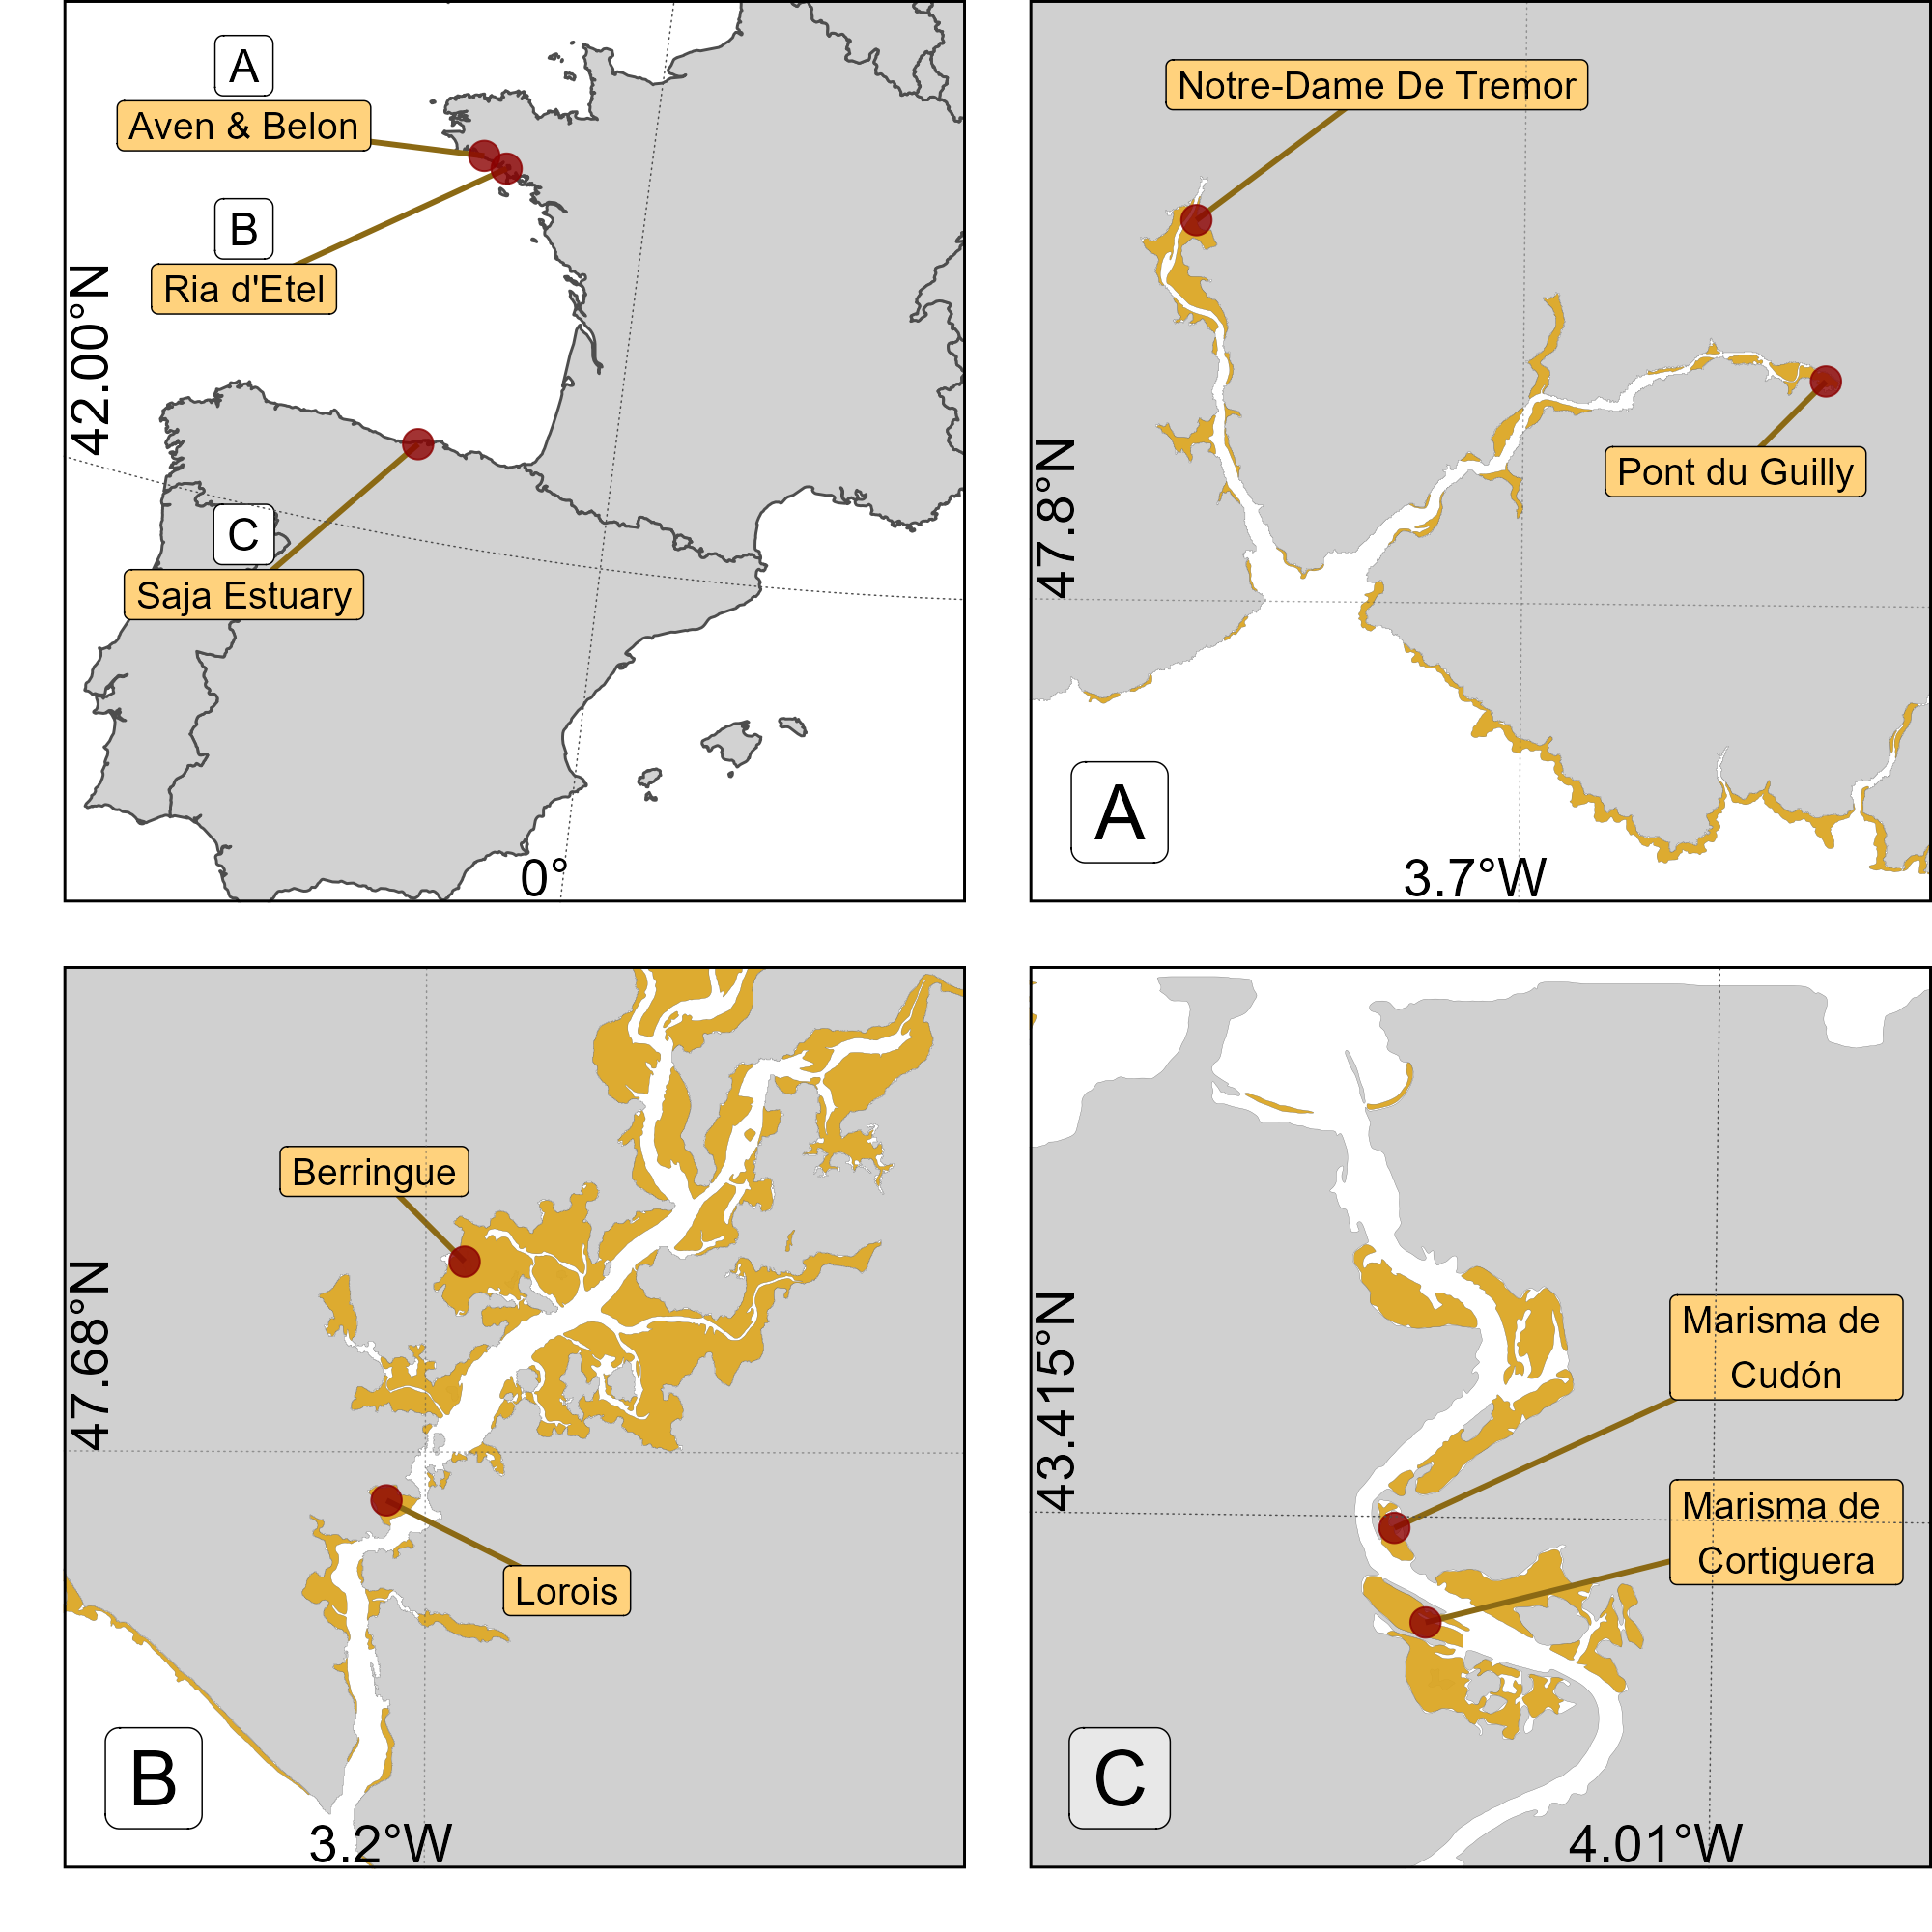
\includegraphics[width=0.95\linewidth,height=\textheight,keepaspectratio]{Figures/Low_res/Figure1/Map_site.png}

}

\caption{\label{fig-location_sites}Location of the drone flights. A:
Flights made in Aven Estuary, France; B: Flights made in Belon Estuary,
France; C: Flights made in the Saja Estuariy, Spain. Golden polygons
represent intertidal areas.}

\end{figure}%

\subsection{Remote sensing data acquisition and
pre-processing}\label{sec-DroneFlights}

\phantomsection\label{cell-fig-PictureFigure}
\begin{figure}[H]

\centering{

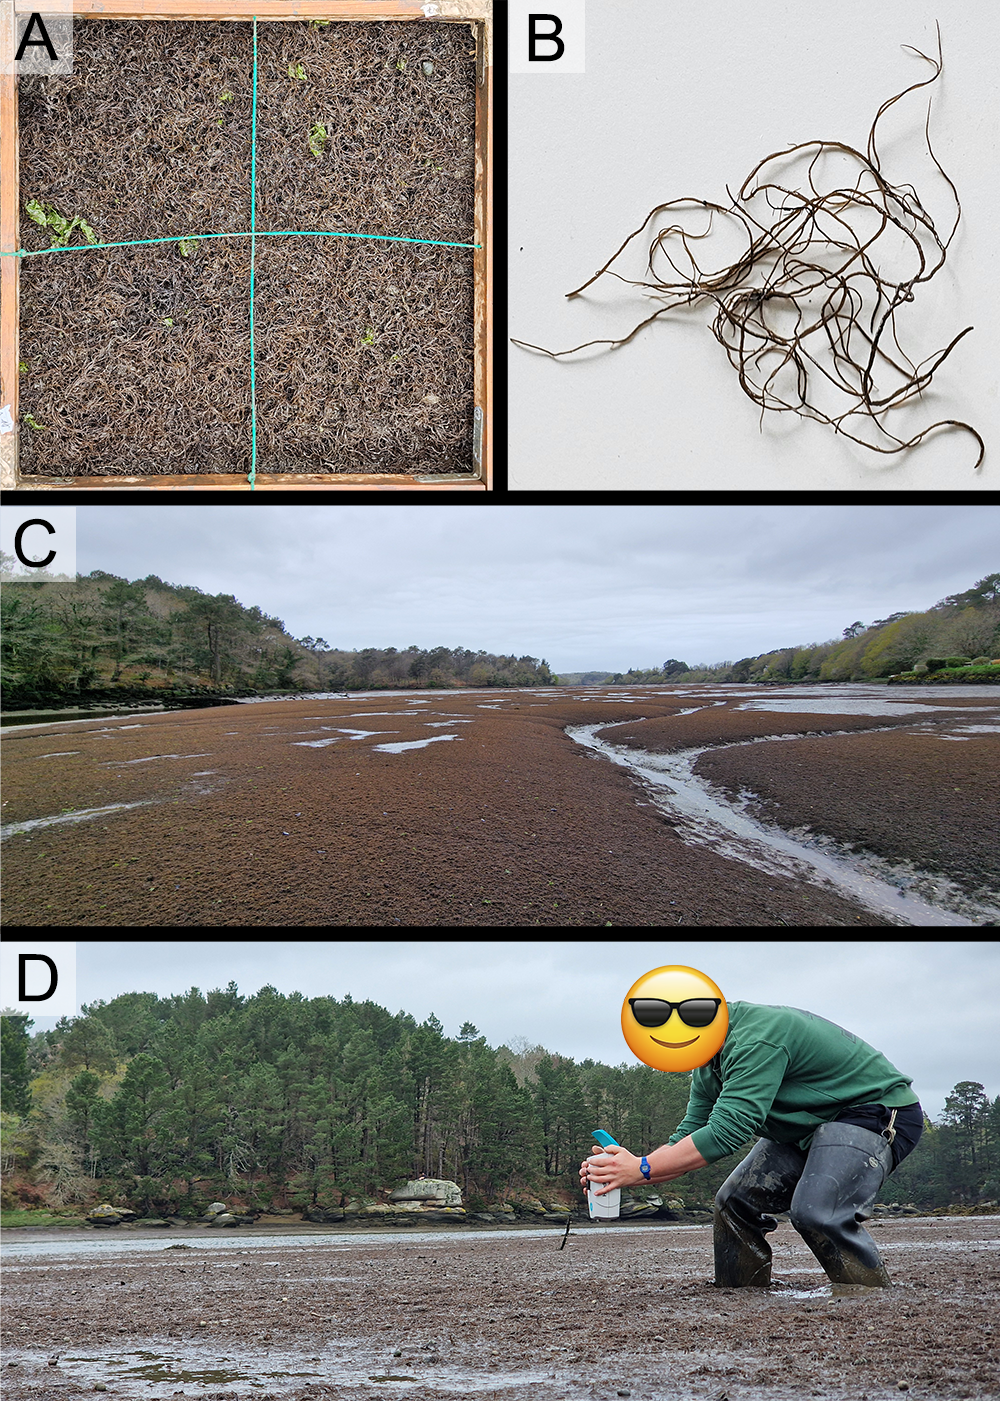
\includegraphics[width=0.95\linewidth,height=\textheight,keepaspectratio]{./Figures/Low_res/FigurePictures_censored.png}

}

\caption{\label{fig-PictureFigure}\emph{Gracilaria vermiculophylla} in
the Belon. A: Quadrat of 0.25 m² with a 100\% cover of \emph{G.
vermiculophylla}; B: Single thallus howing cylindrical branches; C:
Landscape view of mudflats covered by monospecific mats of G.
vermiculophylla; D: Recording of the spectral signature of the algae
using an ASD FieldSpec HandHeld 2 spectroradiometer.}

\end{figure}%

\subsubsection{Hyperspectral
measurements}\label{hyperspectral-measurements}

At each location, hyperspectral reflectance signatures were recorded
using an ASD FieldSpec HandHeld 2 spectroradiometer (Malvern
Panalytical, Worcestershire, UK), which measures reflectance from 325 to
1075 nm with a spectral resolution of approximately 1 nm
(Figure~\ref{fig-PictureFigure} D). Each spectrum was subsequently
smoothed using a Savitzky--Golay filter (Savitzky and Golay, 1964) with
a third-order polynomial and an 11-point window, selected to minimize
noise while preserving salient spectral features. After this initial
smoothing, the first and second derivatives were computed using a
central difference approximation (Equation~\ref{eq-SecondDerivative}).

\begin{equation}\phantomsection\label{eq-SecondDerivative}{
f''(\lambda_i) \approx \frac{f(\lambda_{i+1}) - 2f(\lambda_i) + f(\lambda_{i-1})}{(\Delta \lambda)^2}
}\end{equation}

where \(f(\lambda_i)\) is the reflectance at wavelength \(\lambda_i\)
and \(\Delta \lambda\) is the uniform spectral sampling interval.

\subsubsection{Drone data}\label{drone-data}

A total of four drone flights were conducted across the three study
sites. All flights were performed at an altitude of 120 m and a speed of
10 m·s⁻¹. Two flights were carried out in the Saja Estuary on June 25,
2024, covering areas of 20.4 hectares (Marisma de Cortiguera) and 8.4
hectares (Marisma de Cudón), respectively
(Figure~\ref{fig-location_sites}). The other two flights took place in
the Belon and Aven estuaries on April 11, 2024, covering areas of 21.3
hectares and 26.7 hectares, respectively.

\paragraph{Multispectral data}\label{sec-photo}

At each location, reflectance images with of 1.2 million pixels were
captured using a DJI Matrice 300 quadcopter drone equipped with a
Micasense RedEdge Dual MX multispectral camera. The camera recorded data
across ten spectral bands, spanning from blue to near-infrared (NIR)
wavelengths (444, 475, 531, 560, 650, 668, 705, 717, 740, and 840 nm).
To ensure consistent lighting conditions, the drone's flight trajectory
was aligned to maintain a solar azimuth angle of 90 degrees. Image
acquisition was carried out with an overlap of 70\% between side-by-side
images and 80\% between successive images along the flight path. A
downwelling light sensor (DLS2) was used to measure real-time
irradiance, enabling the correction of reflectance values for variations
in light intensity caused by changing cloud cover during the flight. The
raw image data were subsequently calibrated to reflectance using a
calibration panel with \textasciitilde50\% reflectivity, provided by the
camera's manufacturer. Images were processed using structure-from-motion
photogrammetry software (Agisoft, 2019) to generate multispectral
ortho-mosaics for each flight. The ortho-mosaicking workflow was
consistent across all flights. Initially, key tie points were identified
within each image and across overlapping images to create a sparse point
cloud. This point cloud was refined by removing noisy points using a
reprojection accuracy metric. Subsequently, a dense point cloud was
generated using a structure-from-motion algorithm. A digital surface
model (DSM) was then created through surface interpolation of the dense
point cloud, which served as the basis for reconstructing the
multispectral ortho-image (Nebel et al., 2020). The resolution of the
multispectral ortho-mosaic obtained was 8 cm per pixel.

\paragraph{LiDAR data}\label{lidar-data}

Using the Matrice 300 Series Dual Gimbal Connector, a DJI Zenmuse L1
LiDAR and RGB sensor was mounted on the drone alongside the
multispectral camera. This setup enabled the simultaneous capture of
LiDAR point clouds, high-resolution RGB images, and multispectral images
collected by the MicaSense RedEdge Dual MX during the same flight. The
same processing workflow as Section~\ref{sec-photo} was applied to
process LiDAR RGB images, resulting in ortho-mosaic with a resolution of
2.5 cm per pixel. Since the mapping focused solely on surfaces without
dense vegetation, the LiDAR measured only a single return. Operating in
repetitive scanning mode with a sampling rate of 240 kHz, the system
achieved a point density of 350 points per square meter. The LiDAR point
cloud was extracted and converted into LAS format using DJI Terra
software. The LAS point cloud was then imported into Agisoft Metashape
(Agisoft, 2019) to generate a Digital Surface Model (DSM) with a
resolution of 2.5 cm. From the DSM, the slope of each pixel based on a
grid of 8 surrounding pixels was computed using the terrain function of
the `terra' package in R (Hijmans, 2024). The angle of the mudflat was
categorized into three classes: Flat (angle \textless{} 10°), Angled
(10° ≤ angle ≤ 40°), and Steep (angle \textgreater{} 40°).

\subsection{Scene classification}\label{scene-classification}

In a previous study we developed a neural network classification model
(DISCOV; Oiry et al. (2024)), previously applied with success to
Micasense reflectance data for mapping intertidal vegetation along the
Portuguese and French Atlantic coasts, has been used in this study. The
training dataset of DISCOV v1.0 was updated Figure~\ref{fig-Workflow}.
As shown by Oiry et al. (2024) the DISCOV v1.0 model was trained using
only 5771 Rhodophyceae pixel (3\% of the training dataset). To fill
this, gap the original training dataset of DISCOV v1.0 was updated using
new training pixel coming from the 5 drone flights
(Section~\ref{sec-DroneFlights}). A total of 427000 pixels were added to
the DISCOV training dataset from version 1 (Section~\ref{sec-AnnexeA}).

To validate the DISCOV model, a user-friendly Shiny app was developed.
This app enabled independent users to photo-interpret snapshots of the
ortho-mosaic from each drone flight (Chang et al., 2024; Simon, 2024).
Users could click on various parts of the snapshots to indicate the type
of vegetation they believed was present. Using this method, 3
independent users contributed to creating a validation dataset of 6755
pixels across 79 snapshots distributed among the four drone flights
(Section~\ref{sec-AnnexeB}). The validation dataset was then simplified
into two classes: The presence or absence of Red Algae
(Figure~\ref{fig-Workflow}).

\phantomsection\label{cell-fig-Workflow}
\begin{figure}[H]

\centering{

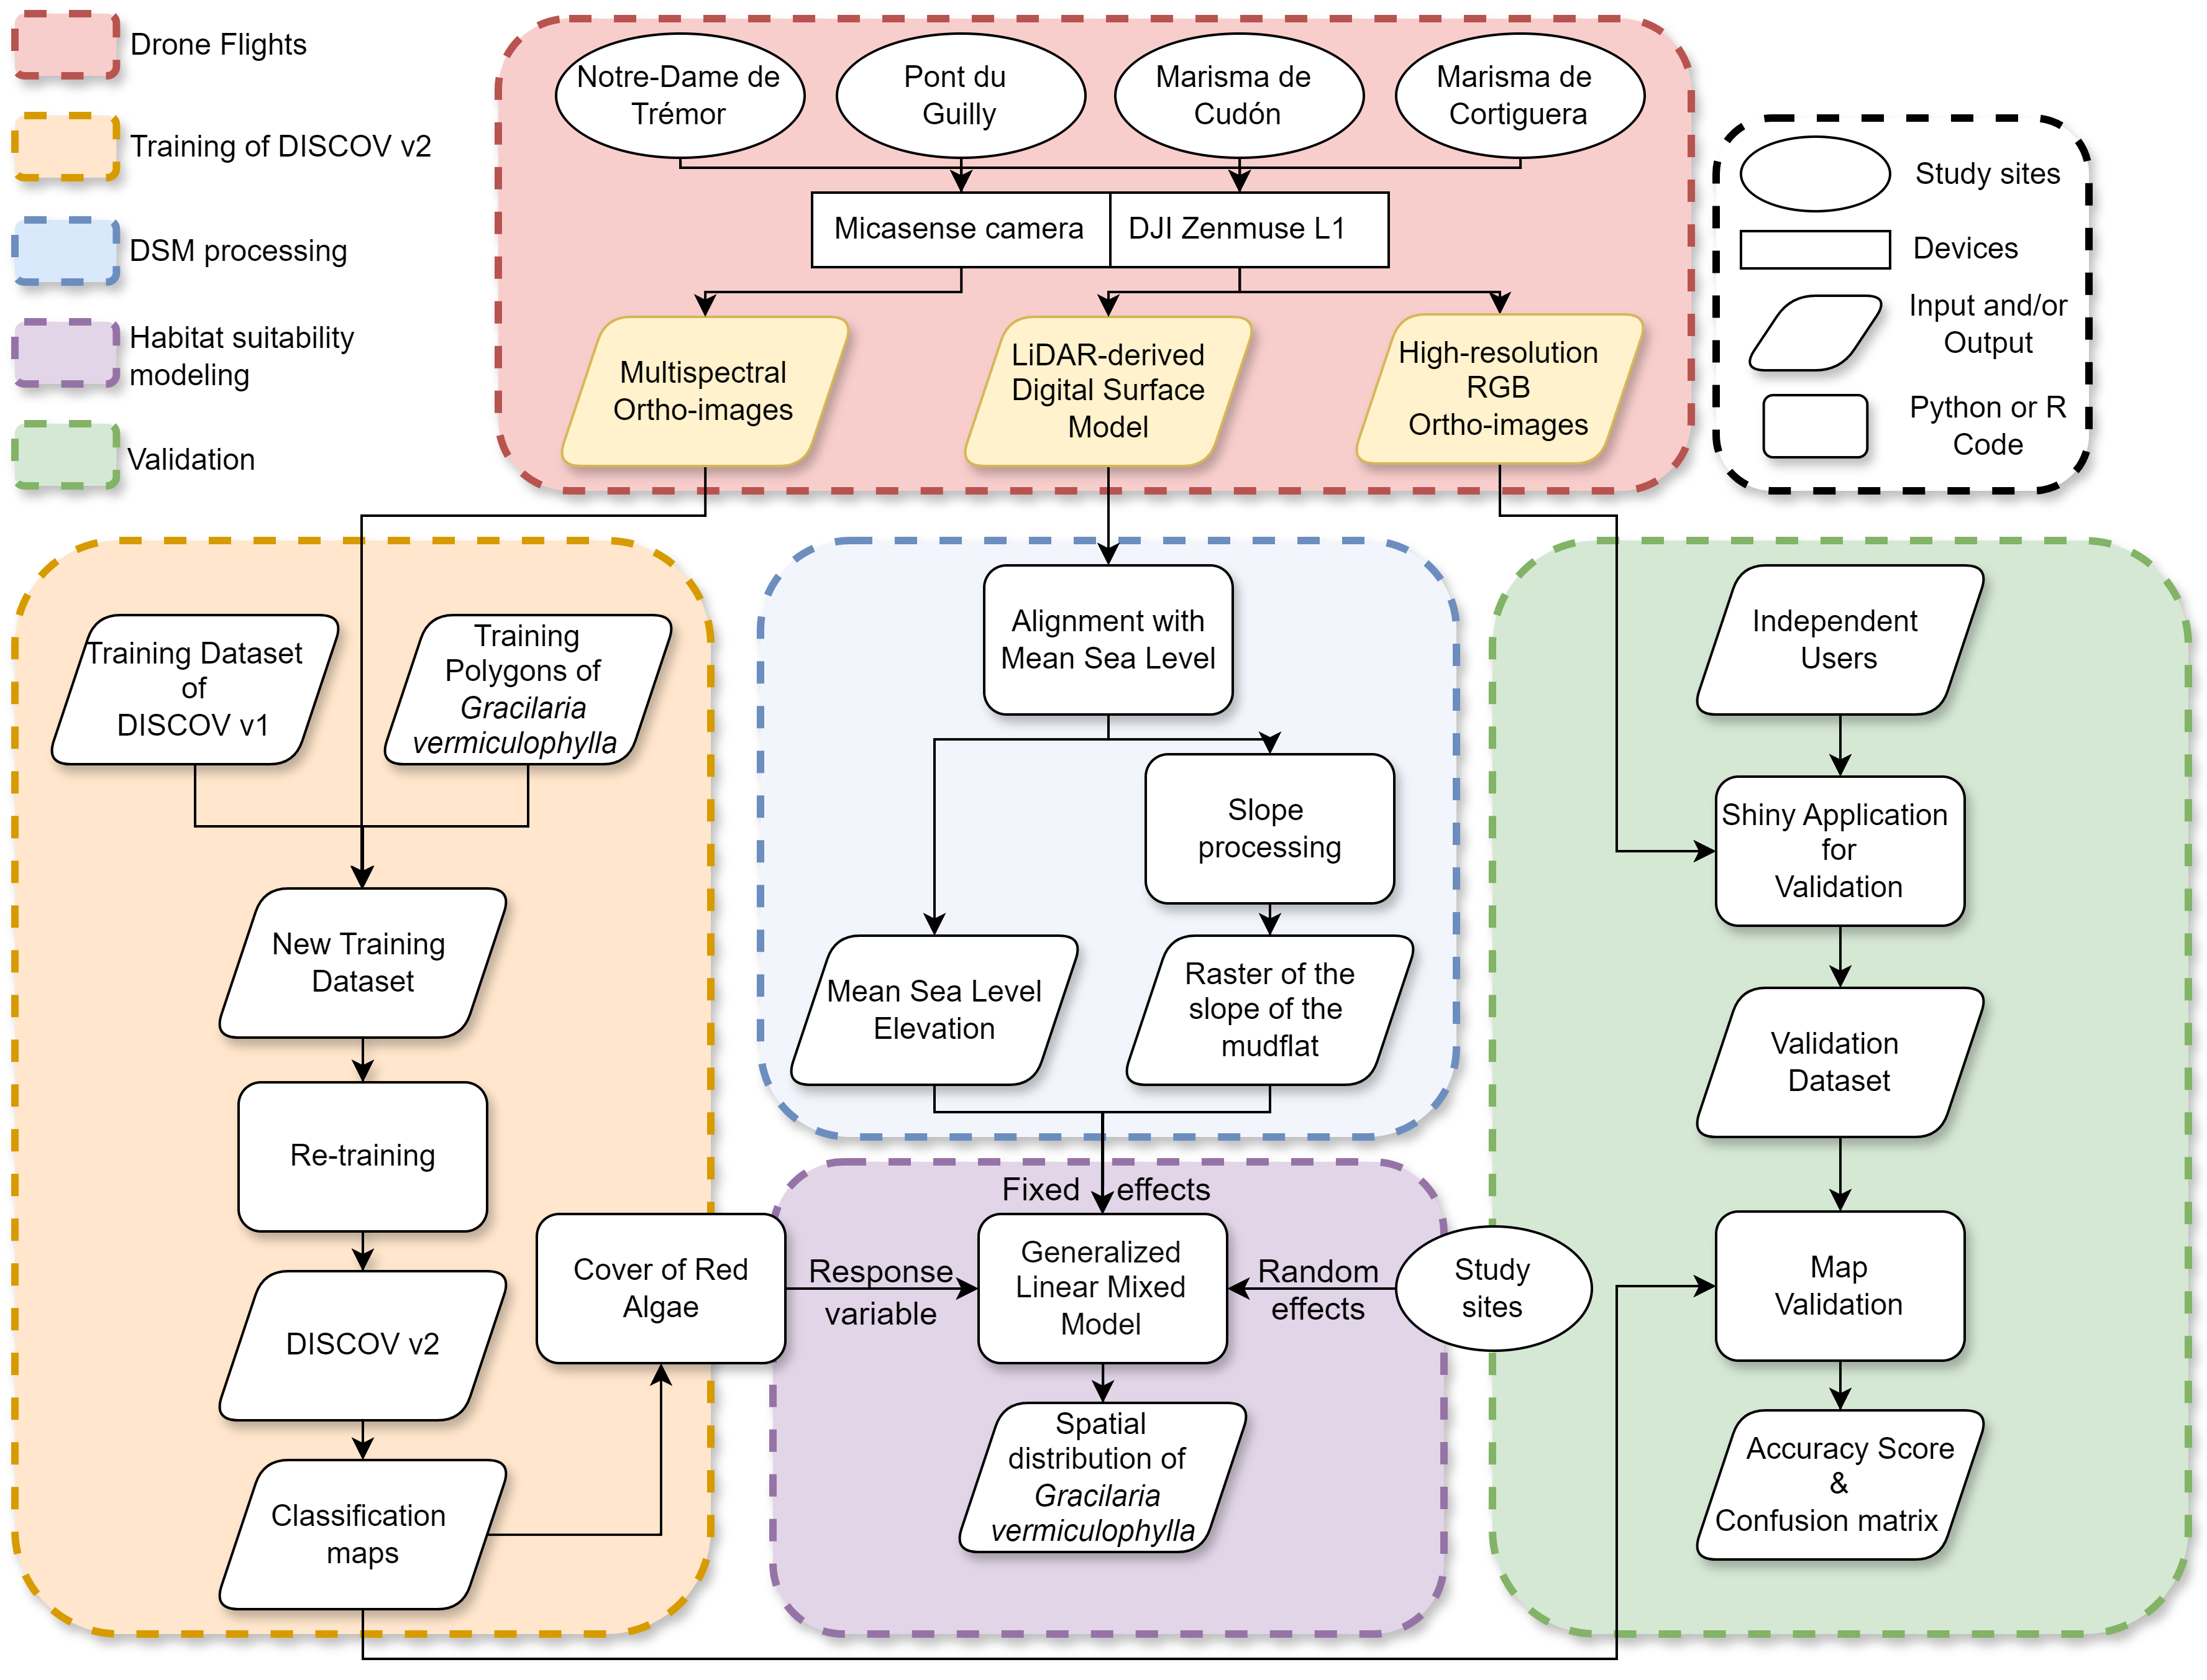
\includegraphics[width=0.95\linewidth,height=\textheight,keepaspectratio]{./Figures/Low_res/Flowchart gracillaria.png}

}

\caption{\label{fig-Workflow}Schematic representation of the workflow.
Parallelograms represent input or output data, rectangles represent
Python processing algorithms, long rectangle represent instruments used
and ovals represent study sites. Red shows Drone data; Orange shows the
model training; Blue shows processing performed on the Digital Surface
Model; Green shows the validation of the model; Purple shows the
statistical analysis.}

\end{figure}%

\subsection{\texorpdfstring{Historical Presence of \emph{Gracilaria
vermiculophylla} in the Bélon
estuary}{Historical Presence of Gracilaria vermiculophylla in the Bélon estuary}}\label{historical-presence-of-gracilaria-vermiculophylla-in-the-buxe9lon-estuary}

To assess the historical presence of \emph{G. vermiculophylla} in the
Belon Estuary, aerial imagery from flight campaigns was obtained via the
IGN platform ``Remonter Le Temps'' (IGN, 2024). Nine images were
selected between 1952 and 2012 from the IGN platform and an additional
one has been added for the year 2024 (Section~\ref{sec-AnnexeC}). Since
most of the images retrieved from ``Remonter Le Temps'' were digitized
versions of physical photographs, georeferencing was required.

For each date, polygons have been drawn around \emph{G. vermiculophylla}
patches by visual photo-interpretation. These polygons were used to
calculate the total area of the mudflat covered by macroalgae within a
common extent of 30 hectares in Pont de Guilly, located in the Belon
Estuary, South Brittany, France.

\subsection{Statistical analysis}\label{statistical-analysis}

We used a Generalized Linear Mixed Model (GLMM) within a Bayesian
framework using the `brms' package in R (Bürkner, 2021, 2018, 2017). The
response variable, the cover of \emph{G. vermiculophylla}, was modeled
using a Beta distribution as a function of bathymetry elevation and the
slope of the mudflat (categorized as Flat, Angled, Steep). A random
intercept for site was included to account for potential hierarchical
variation among sampling sites. The Beta distribution was chosen because
the response variable is continuous and constrained between 0 and 1. We
visually assessed sample vs.~fitted residuals and quartile--quartile
(Q-Q) plots to ensure that the model assumptions, including appropriate
model fit and absence of patterns in residuals, were satisfied.

\section{Results}\label{results}

\subsection{Historical records in the Belon
estuary}\label{historical-records-in-the-belon-estuary}

A clear shift from bare sediment to vegetated mudflats has been observed
over the past 70 years, corresponding to the colonization of the Belon
Estuary by \emph{G. vermiculophylla} (Figure~\ref{fig-HistoricalMap}).
In the 50s, the tidal flats showed no detectable presence of vegetation.
In the 70s some darkening of the sediment became discerbible, but the
first unambiguous presence of \emph{G. vermiculophylla} was 1982. During
the subsequent decades, the cover of algae increased and in 2024, the
high-resolution mapping done with the drone showed that monospecific
mats of \emph{G. vermiculophylla} exclusively colonised the mudflat.

\phantomsection\label{cell-fig-HistoricalMap}
\begin{figure}[H]

\centering{

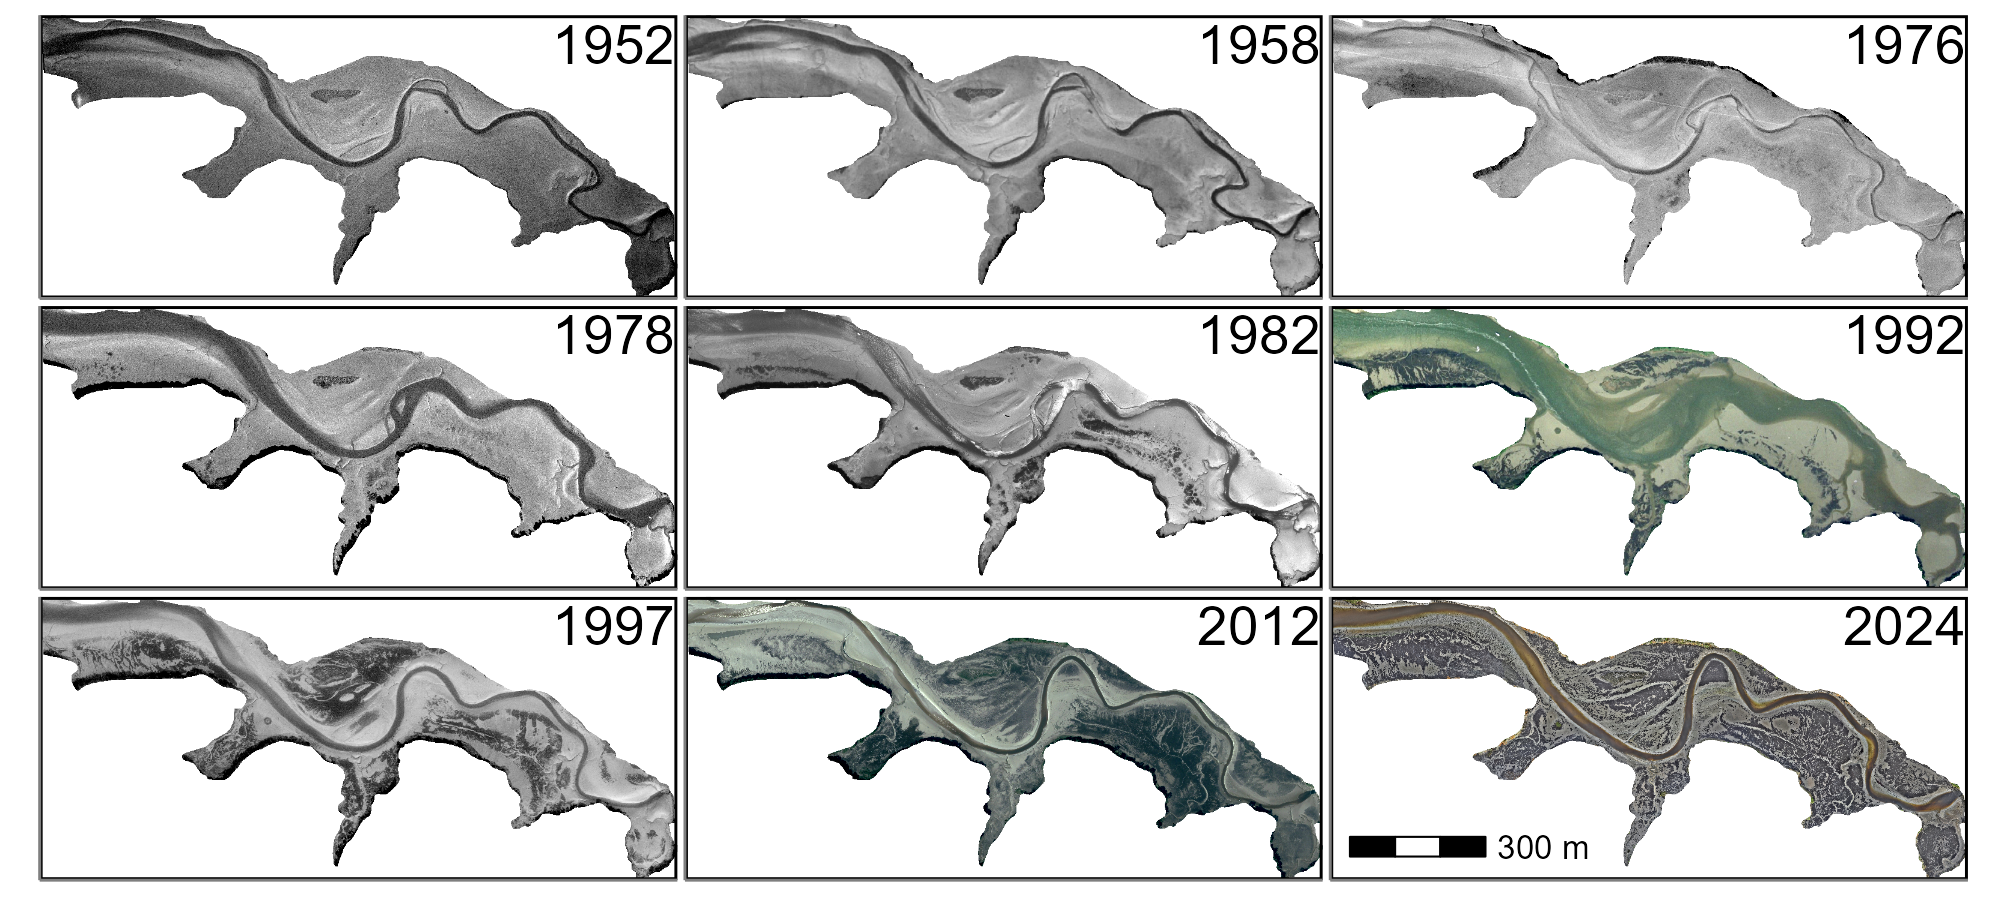
\includegraphics[width=0.95\linewidth,height=\textheight,keepaspectratio]{./Figures/Low_res/Historical_maps.png}

}

\caption{\label{fig-HistoricalMap}RGB images of the Belon Estuary (Pont
de Guilly) showing the colonization of the mudflat by Gracilaria
vermiculophylla between 1952 and 2024.}

\end{figure}%

From the early recordings in the 1950s through the late 1970s,
\emph{Gracilaria vermiculophylla} coverage remained effectively at 0\%
(Figure~\ref{fig-HistoricalPlot}). Shortly after the introduction of
\emph{Crassostrea gigas} in the estuary, in 1971-1972 (see vertical red
dashed line in the figure), the first detectable presence of \emph{G.
vermiculophylla} emerged. By 1976, it covered 2.5\% (0.7 ha) of the Pont
du Guilly area, and by 1978 it had increased slightly to 3.0\% (0.9 ha).
From 1982 onward, coverage expanded more rapidly, increasing from 6.6\%
(2.0 ha) in 1982 to 14.7\% (4.5 ha) in 1992 and nearly 30\% (9.0 ha) by
1997. This upward trend continued into the 21st century, peaking at
41.2\% (13.3 ha) in 2012. Although coverage fluctuated somewhat
thereafter (40.6\% in 2019 and 41.8\% in 2024), it remained consistently
high, indicating sustained and widespread colonization.

\phantomsection\label{cell-fig-HistoricalPlot}
\begin{figure}[H]

\centering{

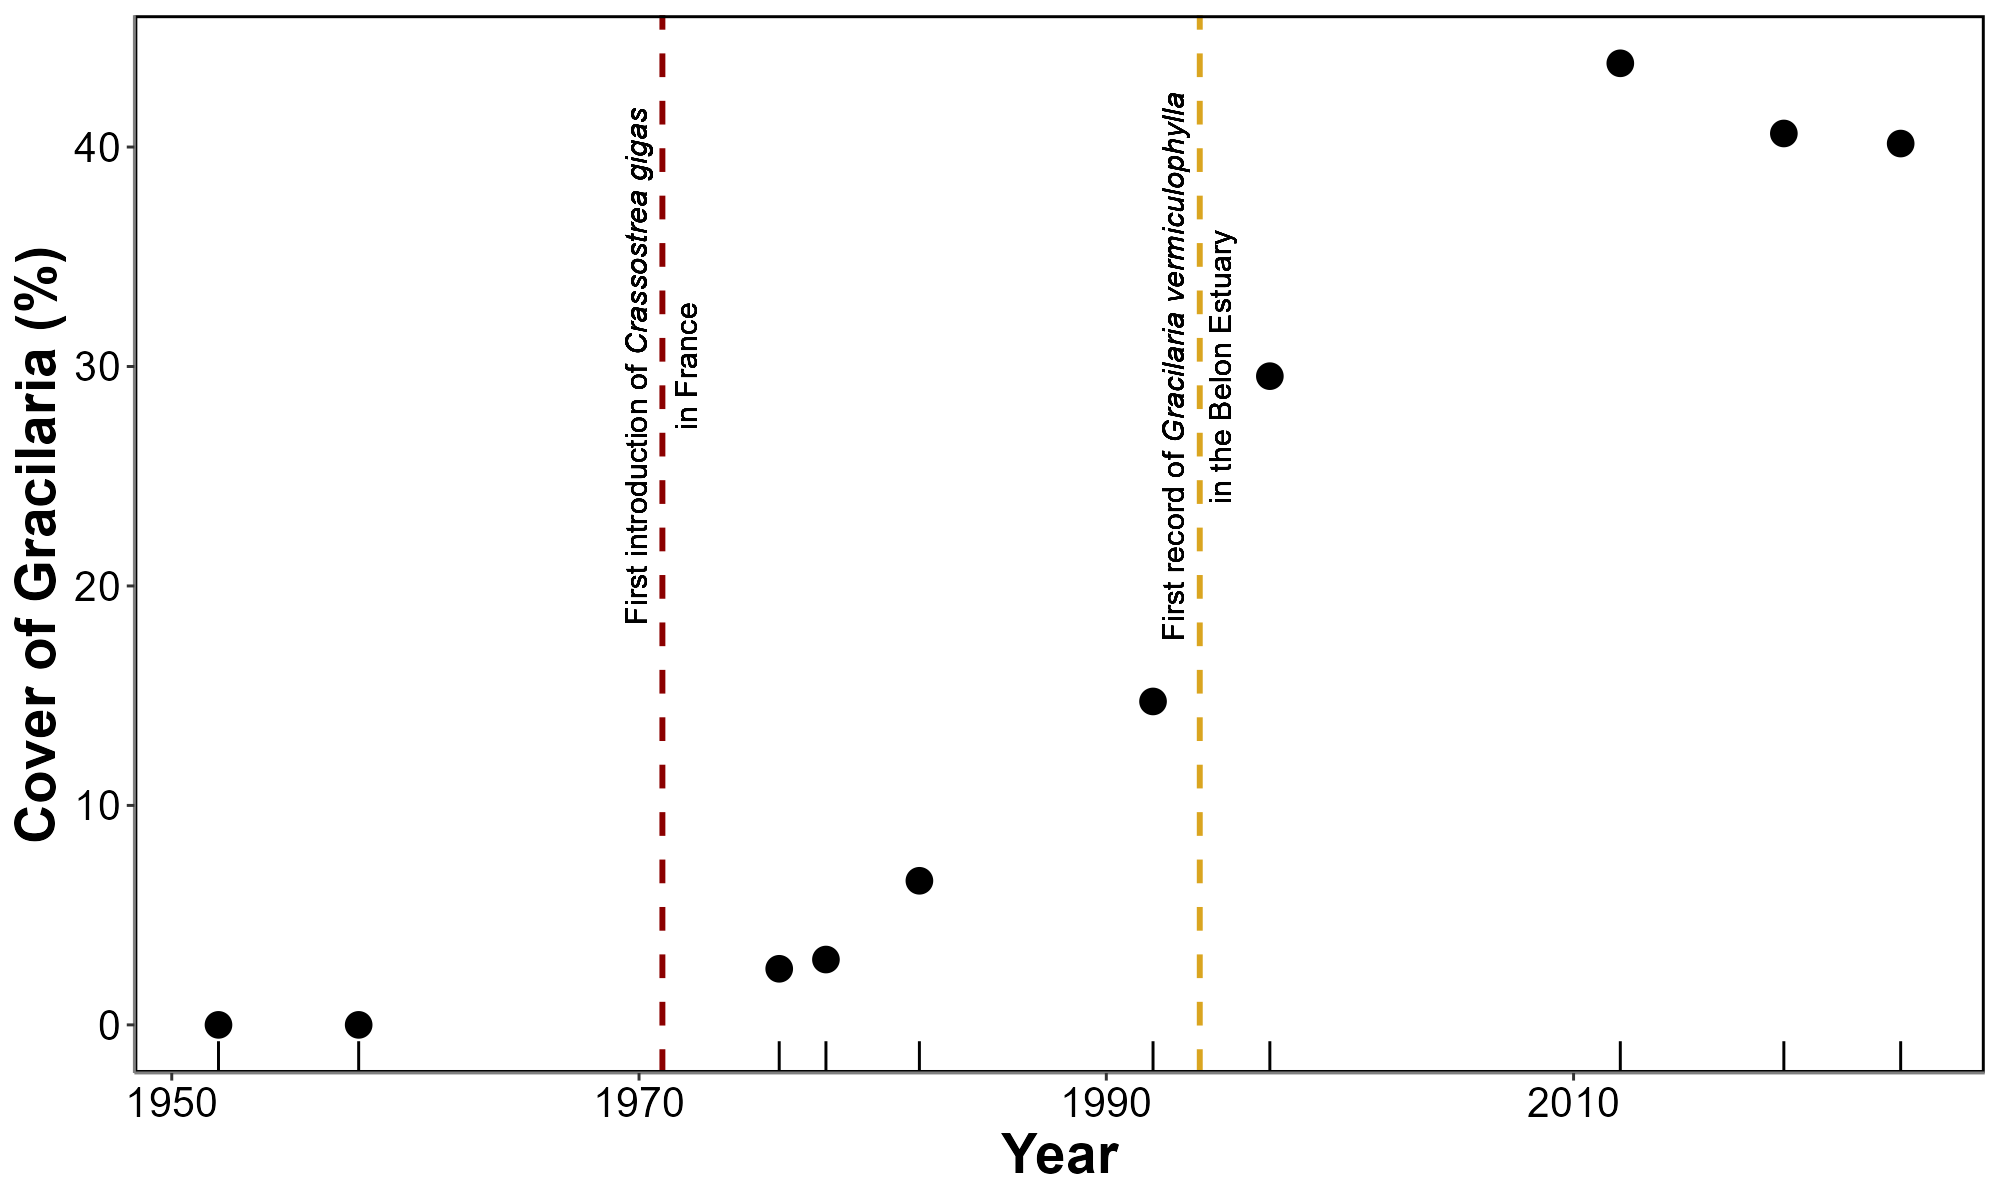
\includegraphics[width=0.95\linewidth,height=\textheight,keepaspectratio]{./Figures/Low_res/Cover_Gracillaria_vs_Time.png}

}

\caption{\label{fig-HistoricalPlot}Trend of the Gracilaria
vermiculophylla cover in the Belon Estuary (at Pont du Guilly). The red
vertical line indicates the date of Crassostrea gigas introduction in
South Brittany (Grizel and Heral, 1991), while the golden line
represents the date of the first documented mention of Gracilaria
vermiculophylla presence in Europe which was in the Belon Esturay
(Rueness, 2005).}

\end{figure}%

\subsection{Spectral description}\label{spectral-description}

The spectral signature of \emph{G. vermiculophylla} was characterized by
a reflectance pattern in the visible region of the spectrum shaped by
the photosynthetic and accessory pigments common to all rhodophytes
(Figure~\ref{fig-SpecDescri} A). This pattern was primarily driven by
phycoerythrin and phycocyanin, which exhibited maximum absorption peaks
at approximately 565 nm and 620 nm, respectively. An additional
absorption feature around 495 nm was likely attributable to accessory
carotenoid pigments. The most pronounced absorption peak occurred at 675
nm, corresponding to chlorophyll-a absorption. The second derivative
analysis clearly highlighted the inflection points corresponding to the
main absorption peaks at 495, 565, 620, and 675 nm, allowing for more
precise identification of the wavelength associated with these pigments
(Figure~\ref{fig-SpecDescri} B).

\phantomsection\label{cell-fig-SpecDescri}
\begin{figure}[H]

\centering{

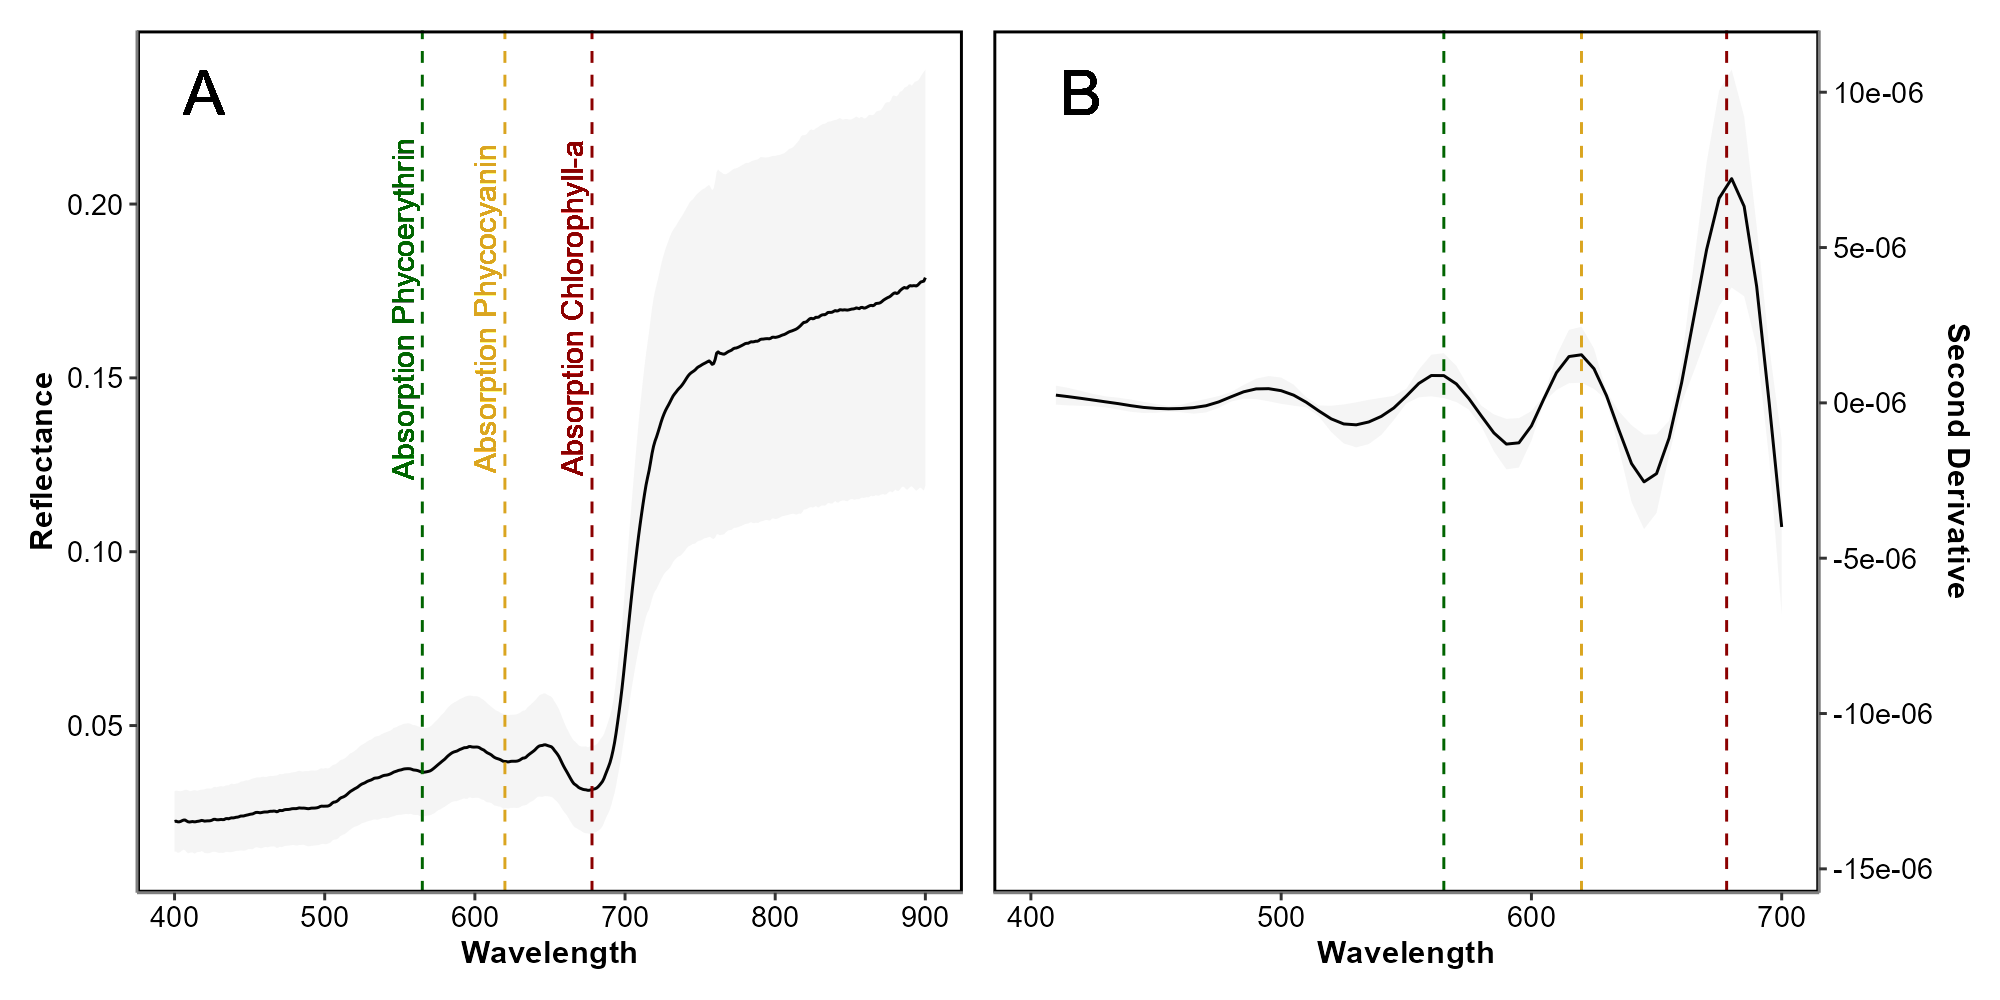
\includegraphics[width=0.95\linewidth,height=\textheight,keepaspectratio]{./Figures/Low_res/plot_spectral_signature.png}

}

\caption{\label{fig-SpecDescri}Hyperspectral signature of
\emph{Gracilaria vermiculophylla} (A) and its second derivative (B). The
black line represents the average spectra, while the shaded area
indicates the standard deviation. Dashed lines mark the absorption
maxima of Phycoerythrin, Phycocyanin, and Chlorophyll-a, shown in green,
orange, and red, respectively.}

\end{figure}%

\subsection{Spatial distribution}\label{spatial-distribution}

The classification map obtained from the neural network algorithm is
shown for the Belon estuary (Figure~\ref{fig-Belon} A). Among the main
classes of the intertidal vegetation, the class fo Rhodophyceae (red
macroalgae, in red) was the dominant algal cover, forming extensive,
continous patches colonizing almost the entire mudflat. In contrast,
Bacillariophyceae (diatoms biofilm, in orange) and Chlorophyceae (Green
macroalgae, in green) exhibited more localized distributions, typically
restricted to smaller, fragmented patches. A few Phaeophyceae (brown
macroalgae, in brown) were confined to limited patches in the upper
intertidal attached to rocks. In the Saja esturay, Rhodophyceae cover
was more scarsed, due to a strong Chlorophyceae presence on this site
(Annexe D: Section~\ref{sec-AnnexeD}).

Across the study sites the presence/absence of \emph{G. vermiculophylla}
was classified with a global accuracy of 91.1 \%, a sensitivity of 96.5
\% and a specificity of 71.5 \%.

The elevation map showed that the main mats of G. vermiculophylla were
between 1 and 2 m above mean sea level (Figure~\ref{fig-Belon} C). Algal
presence was markedly elevation-driven, with lower intertidal zones
closer to the tidal channel consistently exibiting reduced macroalgal
cover. Most of the intertidal flats exibited slope below 10° (Violet,
(Figure~\ref{fig-Belon} D). Angled surfaces (10° \textless{} Slope
\textless{} 40°) often found next to tidal channels were exibiting
almost no vegetation cover.

\phantomsection\label{cell-fig-Belon}
\begin{figure}[H]

\centering{

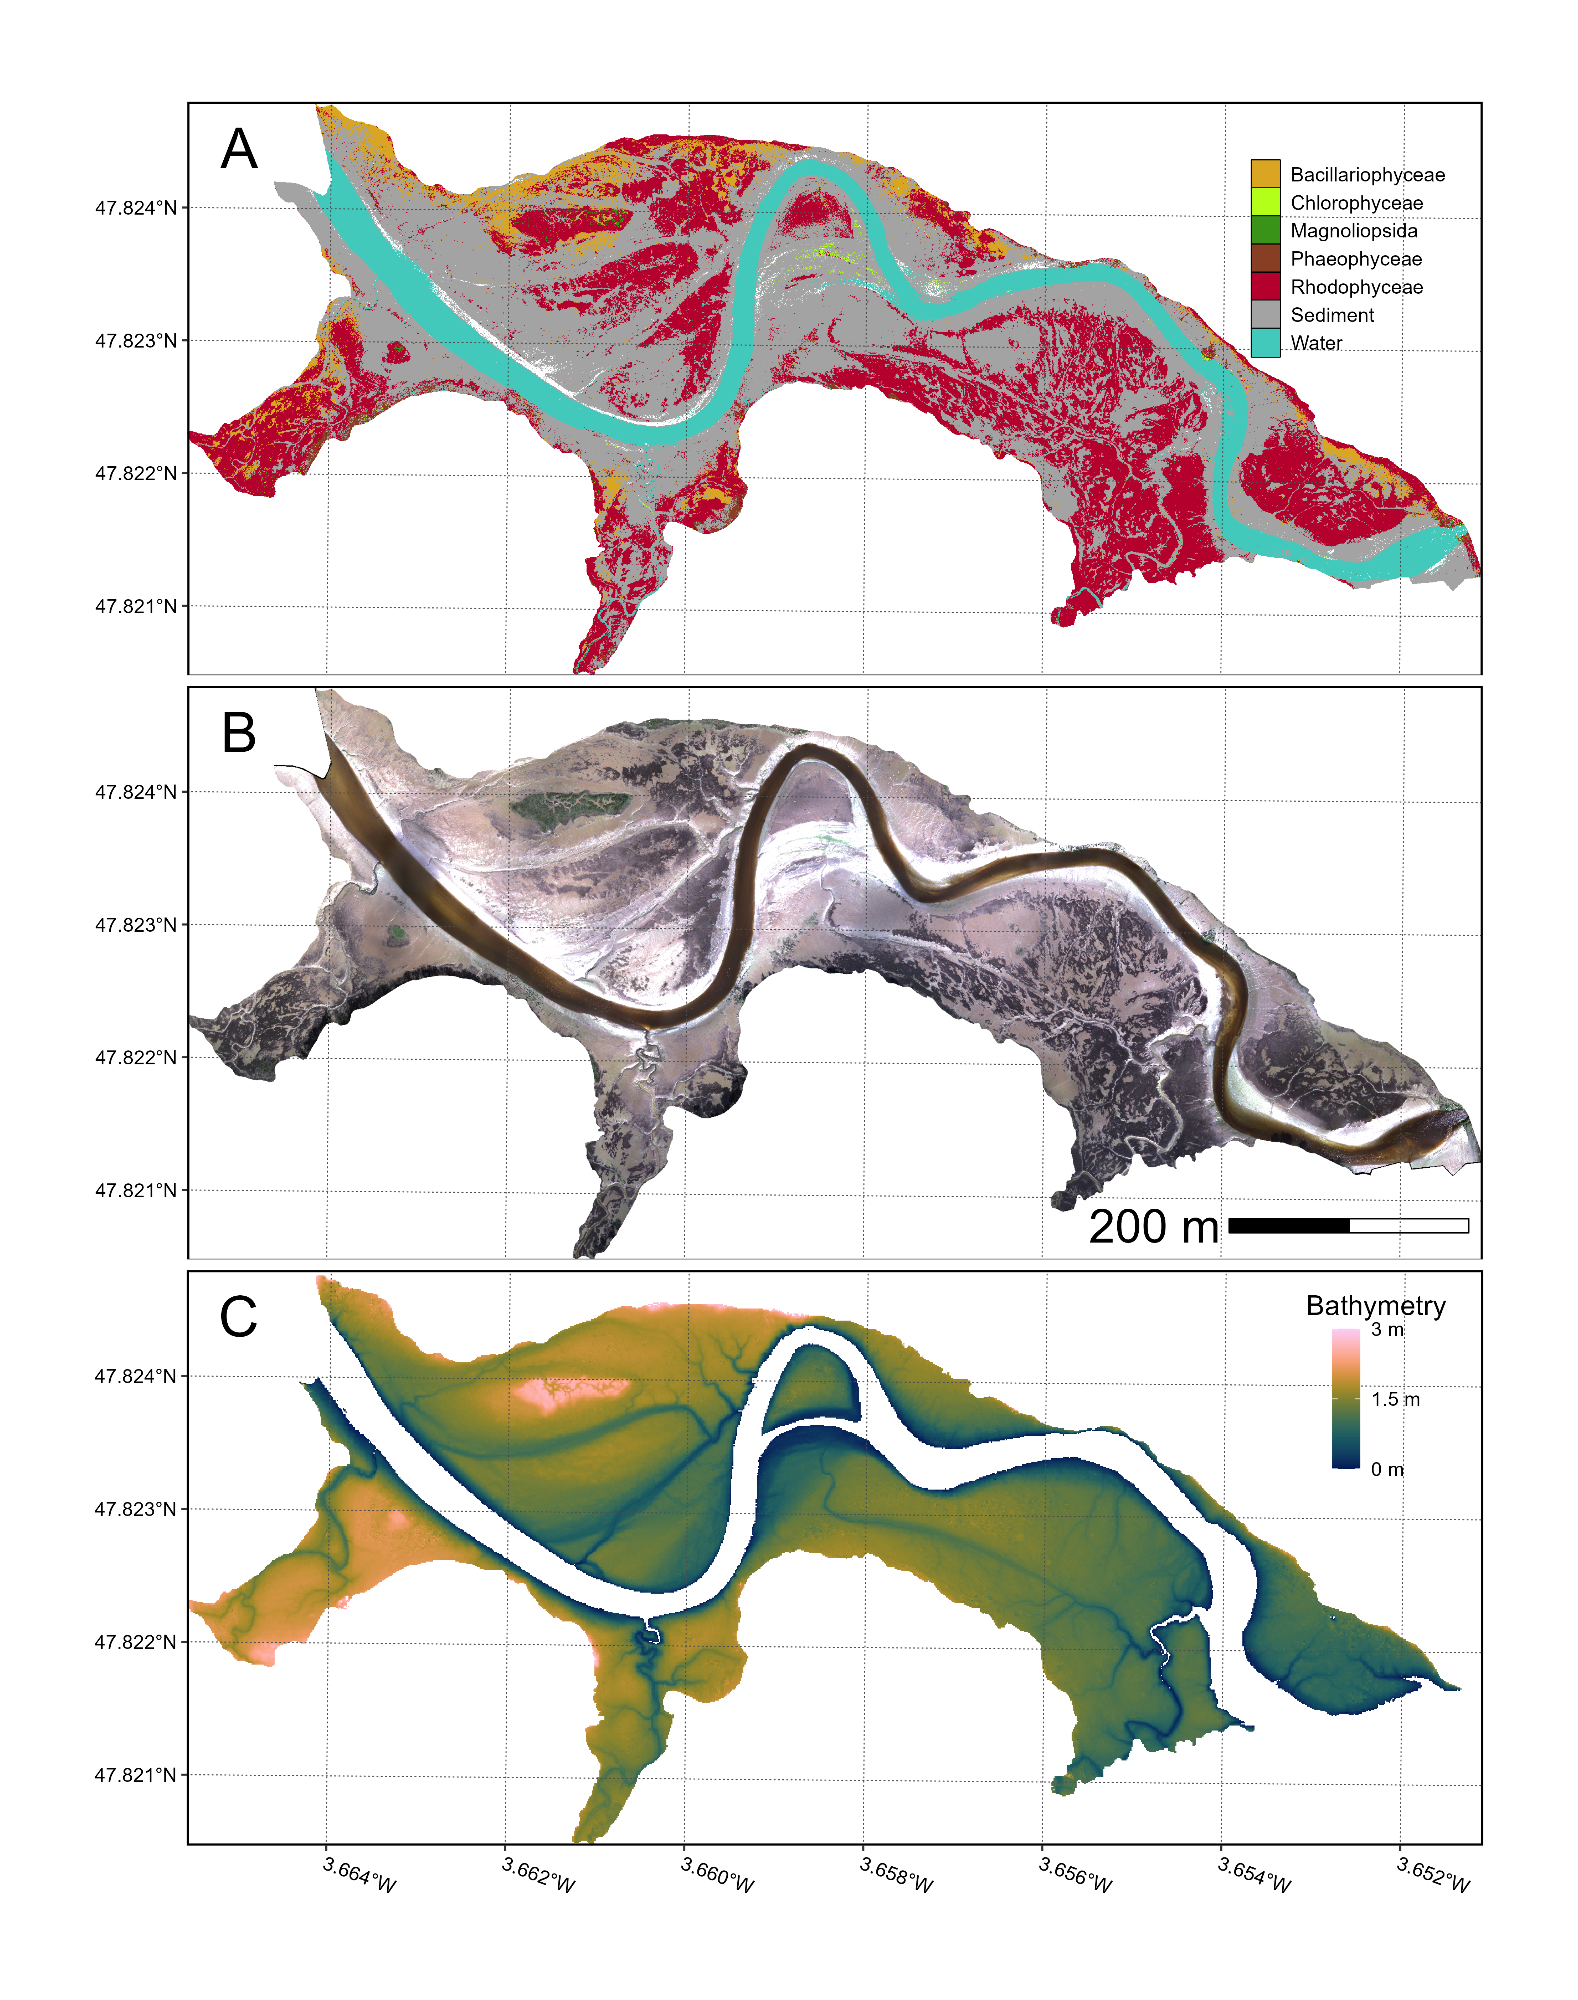
\includegraphics[width=3.75in,height=\textheight,keepaspectratio]{./Figures/Low_res/Belon_maps.png}

}

\caption{\label{fig-Belon}Classification of the main classes of
intertidal vegetation with a neural network algorithm (A), RGB
composition (B), Elevation (C) and mudflat topography (D) of the Belon
estuary site in Brittany, France. The total extent of this flight was 21
hectares with a resolution of 8 mm per pixel. Elevation corrsponds to
the height above mean sea level.}

\end{figure}%

Overall, the percent cover of \emph{G. vermiculophylla} increased with
elevation, as shown by the general relationship
(Figure~\ref{fig-Gam_Slope}, black line), which rises from approximately
16\% at the lowest elevation to about 30\% at the highest elevation.
This indicates a consistent positive association between elevation and
algal cover.

When accounting for slope, the flatter the slope, the higher the percent
cover of \emph{G. vermiculophylla}. For flat slopes, the cover ranged
from approximately 20\% at the lowest elevation to nearly 38\% at the
highest elevation. In contrast, the increase was less pronounced for
angled slopes, ranging from around 16\% to 32\%. The cover was the
lowest on steep slopes, starting at about 15\% and rising only slightly
above 30\% at the highest elevation (Figure~\ref{fig-Gam_Slope}). This
demonstrates that slope modifies the relationship, with flatter slopes
supporting a greater percent cover of the algae.

\phantomsection\label{cell-fig-Gam_Slope}
\begin{figure}[H]

\centering{

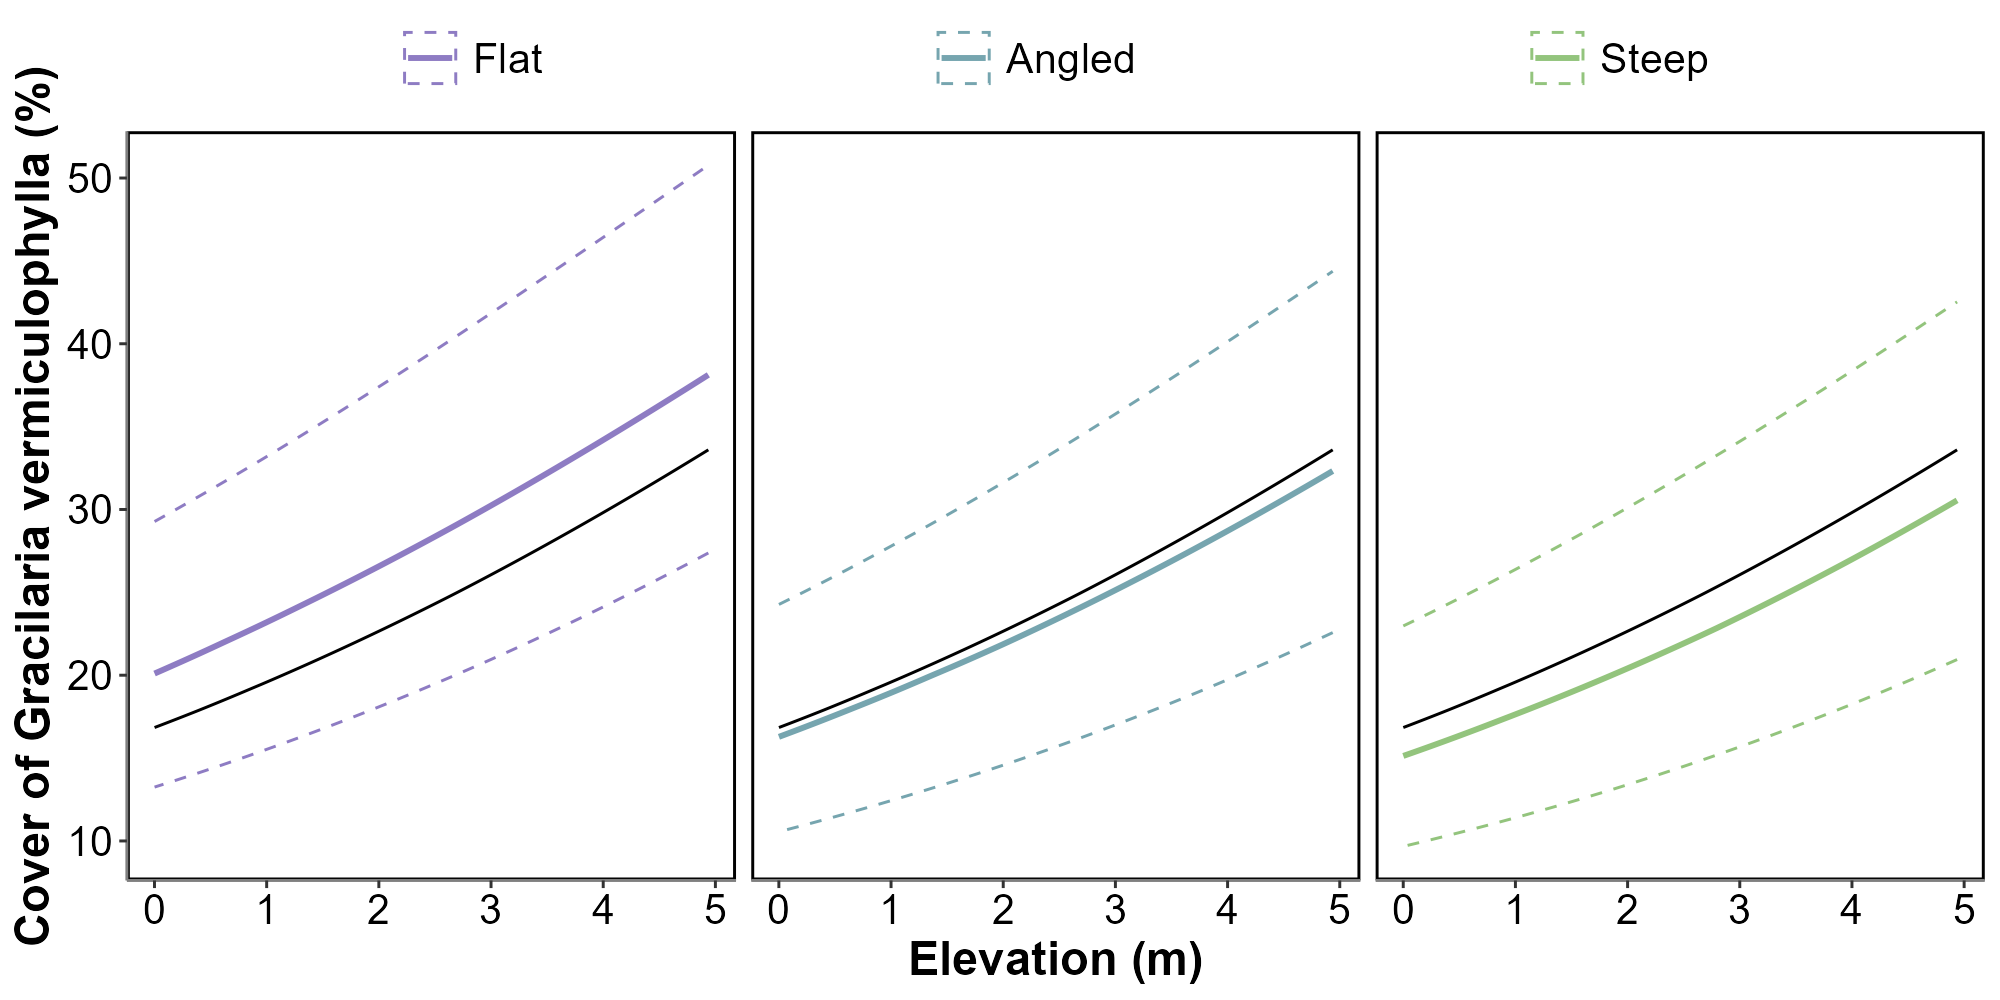
\includegraphics[width=0.95\linewidth,height=\textheight,keepaspectratio]{./Figures/Low_res/GAM_slope_cover.png}

}

\caption{\label{fig-Gam_Slope}DISCOV Prediction (A), RGB composition (B)
and Bathymetry (C) of the Bélon estuary site in Brttany, France. The
total extent of this flight was 21 hectars with a resolution of 8 mm per
pixel. Bathymetry is represented as the height above mean sea level.}

\end{figure}%

\section{Discussion}\label{discussion}

\subsection{\texorpdfstring{Drone mapping \emph{G. vermiculophylla} with
machine
learning}{Drone mapping G. vermiculophylla with machine learning}}\label{drone-mapping-g.-vermiculophylla-with-machine-learning}

In this study, we produced the first spatial distribution maps of the
invasive red alga \emph{Gracilaria vermiculophylla} using a
multispectral drone survey conducted at low tide in Atlantic estuaries
representing varied environmental conditions. In southern Brittany, the
species formed monospecific mats, while in the Cantabrian region of
Spain, it was intermixed with other intertidal vegetation.
Distinguishing among these vegetation types was a key prerequisite for
the analysis.

To achieve this, we adapted the deep learning-based classification model
DISCOV (Oiry et al., 2024), initially developed to discriminate seagrass
from green macroalgae. Although the original model included Rhodophyceae
as a class, this group constituted less than 3\% of its training
dataset. In contrast, the updated model presented here was trained on a
dataset in which \emph{G. vermiculophylla} covered 26 \% of
approximately one million pixels. This improved dataset allowed the
model to achieve an accuracy of 91.1 \%.

Rhodophytes possess unique phycobilin pigments, enabling their spectral
distinction from other macroalgal groups (Douay et al., 2022; Mcilwaine
et al., 2019; Olmedo-Masat et al., 2020). Even with the ten-band
multispectral sensor used in our study, it remained feasible to
discriminate the major classes of intertidal macrophytes (Davies et al.,
2023; Oiry et al., 2024; Román et al., 2021). However, the model
identifies \emph{G. vermiculophylla} at the class level (Rhodophyceae)
rather than at the species level. Although hyperspectral approaches may
allow finer taxonomic resolution (Douay et al., 2022; Olmedo-Masat et
al., 2020), it is unlikely that Gracilaria species can be precisely
distinguished using standard multispectral sensors.

Ecological factors also aid in differentiating \emph{G.
vermiculophylla}. Unlike many other macroalgae that require hard
substrates, \emph{G. vermiculophylla} establishes itself on soft-bottom
sediments. In fact, it is commonly found on mudflats, anchoring its
thalli in the top 10 cm of mud (Surget, 2017), and inhabits the upper
intertidal zone---an unusual trait for a Rhodophyte (Abreu et al., 2011;
Davoult et al., 2017). By reliably detecting \emph{G. vermiculophylla}
in these soft-substrate, upper intertidal habitats, our method provides
a framework for identifying environmental conditions that favor its
spread, potentially offering managers early-warning indicators to
control its expansion before it reaches nuisance levels. Thus, combining
spectral data with sediment characteristics provides a strong indicator
of \emph{G. vermiculophylla} presence in European Atlantic estuaries,
complementing the physical variables already used in species
distribution modeling (Mendoza-Segura et al., 2023).

In addition, the scalability of drone-based surveying facilitates repeat
mapping to detect temporal shifts in the distribution and abundance of
\emph{G. vermiculophylla.} Such continuous monitoring could capture
seasonal patterns of colonization, allowing researchers and
environmental managers to evaluate the effectiveness of mitigation
measures, track long-term ecological impacts, and anticipate future
shifts in habitat suitability under changing climate conditions.

\subsection{\texorpdfstring{\emph{G. vermiculophylla} spatial
distribution and mudflat
topography}{G. vermiculophylla spatial distribution and mudflat topography}}\label{g.-vermiculophylla-spatial-distribution-and-mudflat-topography}

The spatial distribution of \emph{G. vermiculophylla} across intertidal
zones reveals a distinct relationship with mudflat topography, which
significantly influences algal density and coverage. Our results show
that higher elevations within the intertidal zone support greater
densities of \emph{G. vermiculophylla}. A pattern that aligns with
findings by Thomsen et al. (2009), where elevated areas provided optimal
conditions for algal survival. \emph{G. vermiculophylla} demonstrates
remarkable physiological plasticity, enabling it to tolerate a broad
spectrum of environmental conditions, including temperature fluctuations
(Sotka et al., 2018), nutrient variability (Abreu et al., 2011), and a
wide range of salinities (Weinberger et al., 2008). Its capacity for
sustained growth under low salinity conditions (Nyberg, 2007; Rueness,
2005) underpins its successful establishment and persistence within
polyhaline and mesohaline estuarine environments. A strong constrain,
however, for the algae is the hydrodynamism. Unlike seagrasses, another
type of marine plant that can also colonize soft sediment, which possess
rhizomes that provide robust anchorage, \emph{G. vermiculophylla} lacks
such specialized structures. Its attachment to the substrate relies
solely on its buried thalli, which embed into the upper layers of soft
sediment. This mode of anchorage renders the alga particularly
vulnerable to high hydrodynamic conditions, as it lacks the structural
stability needed to withstand strong currents or wave action. To
partially bury its thalli into the sediment, \emph{G. vermiculophylla}
requires areas with high sedimentation rates. These conditions are
typically found in the upper regions of estuarine systems or in
proximity to other macrophytes, such as \emph{Sporobolus} spp. (commonly
known as small cordgrass), which reduce current velocity and promote
sediment deposition (Mudd et al., 2010). This observation aligns with
the findings illustrated in Figure~\ref{fig-HistoricalMap}, which show
that one of the first areas colonized by \emph{G. vermiculophylla} in
1992 in the Bélon estuary, France, was located near a patch of salt
marsh.\\
As a result, \emph{G. vermiculophylla} compensates for its vulnerability
to hydrodynamic forces by forming dense mats, which enhance its
stability and facilitate its persistence and proliferation in intertidal
and estuarine environments with low to moderate hydrodynamic conditions
(Surget, 2017).

The negative relationship between slope steepness and the density of
\emph{G. vermiculophylla} can be explained by the physical and
ecological characteristics of steeper mudflat areas. Steeper slopes are
typically associated with higher rates of water runoff during tidal
exchanges, resulting in stronger hydrodynamic forces. These forces can
lead to increased sediment erosion, reduced sedimentation, and less
stable substrate conditions, which are unfavorable for \emph{G.
vermiculophylla} to anchor its thalli effectively (Besterman et al.,
2021). Furthermore, steeper slopes may limit the retention of organic
matter and nutrients, reducing the availability of essential resources
needed for algal growth. In contrast, flatter areas within the
intertidal zone are more likely to accumulate fine sediments and retain
water for longer durations during low tides, creating a more stable and
nutrient-rich environment conducive to \emph{G. vermiculophylla}
proliferation. Additionally, these conditions may favor the formation of
dense algal mats, which further stabilize the sediment and promote
growth.

\subsection{\texorpdfstring{Monitoring \emph{Gracilaria vermiculophylla}
Invasion
Dynamics}{Monitoring Gracilaria vermiculophylla Invasion Dynamics}}\label{monitoring-gracilaria-vermiculophylla-invasion-dynamics}

The invasive red alga \emph{G. vermiculophylla} represents a significant
example of delayed recognition and documentation in biological
invasions. Historical aerial imagery and photo-interpretation analyses
from the Bélon Estuary suggest the initial presence of this species in
1976 Figure~\ref{fig-HistoricalMap}, preceding its first formal
description in European waters in 1996 by two decades (Rueness, 2005).
This delay likely stems from insufficient early monitoring frameworks
and limited awareness of its ecological impacts, which often
characterize the early stages of invasive species colonization. It also
arises from the fact that others red macroalgae species, resembling
\emph{G. vermiculophylla} and native to this area (e.g.~\emph{Gracilaria
gracilis}) were already present at sites where \emph{G. vermiculophylla}
was introduced, further complicating its detection. This lag highlights
challenges associated with the detection, monitoring, and reporting of
invasive species and their ecological impacts during early colonization.

The appearance of \emph{G. vermiculophylla} in 1976 corresponds with the
introduction of the Pacific oyster (\emph{Crassostrea gigas}) into the
estuary, a few years before, between 1971 and 1975, and a potential
vector for algal dispersal through aquaculture activities (Grizel and
Heral, 1991; Rueness, 2005). Aquaculture practices, such as the transfer
of oyster spat and equipment between regions, facilitate the
unintentional transport of invasive algal fragments. For instance,
\emph{G. vermiculophylla} may have attached to shells or nets used in
oyster farming, enabling its spread to new estuarine habitats. After
initial establishment, the alga progressively occupied suitable
habitats, consistent with theoretical invasion dynamics involving a lag
phase followed by rapid spread (Arim et al., 2006). The establishment of
\emph{G. vermiculophylla} likely induced changes in sediment
characteristics, trophic interactions, and habitat structure prior to
formal recognition (BenDor and Metcalf, 2006). Such shifts are
comparable to documented impacts in similar systems (Crowl et al., 2008;
Gallardo et al., 2016), yet remain difficult to quantify without early
monitoring data. Remote sensing using multispectral drone mapping can
provide high-resolution, spatially explicit data, but it must be
combined with repeated, \emph{in situ} field measurements to maximize
its potential (Chadwick et al., 2020; Zoffoli et al., 2023). Temporal
repetition makes it possible to assess dynamic processes, and
integrating these mapping approaches with \emph{in situ} analyses of
local infauna, carbon cycling, riverine inputs, and sedimentology yields
valuable data for local managers. Such an integrated approach can
determine how the invasive algae affects the local ecosystem and, more
broadly, forecast its potential impact on other estuarine environments
facing similar invasion events.

The temporal gap between the first presence and documentation reflects
limitations in early surveillance, potentially underestimating
ecological and economic impacts during the initial colonization phase.
Studies on invasion dynamics demonstrate that early detection is crucial
for effective containment and management, particularly before an
invasion reaches the exponential spread phase, which complicates control
efforts (Arim et al., 2006; BenDor and Metcalf, 2006; Elton, 2020).
Specific practices, such as the removal of early-stage algal mats,
implementation of physical barriers to prevent further spread, and
public awareness campaigns, could mitigate the impacts during this
critical phase (Green and Grosholz, 2021; Jones et al., 2021;
Simberloff, 2021). In the Bélon Estuary, \emph{G. vermiculophylla}
appears to have thrived under ecological conditions favorable to its
proliferation, enabling the formation of dense mats in about 6 years
(between 1976 and 1982; Figure~\ref{fig-HistoricalMap}) after its first
detection in the estuary. This undocumented growth likely contributed to
substantial changes in the estuarine ecosystem. Historical aerial
imagery has provided valuable insights into long-term invasion patterns
by enabling the retrospective identification of shifts in habitat
characteristics. Modern drone-based systems enhance this capacity
through high spatial and temporal resolution, enabling the rapid
detection of invasive species at early stages of establishment. By
capturing detailed data on the spatial distribution and habitat
preferences of species such as \emph{G. vermiculophylla}, remote sensing
facilitates timely interventions, allowing stakeholders to take rapid
measures to limit the invasion. Integrating these tools into routine
monitoring programs offers a scalable and efficient means to track
invasive species dynamics and inform targeted management strategies,
such as habitat restoration, removal of invasive mats, and prevention of
further spread through targeted interventions. Expanding these
methodologies to lower-cost RGB-based detection would further
democratize access to monitoring tools, enabling more widespread
application for early detection and rapid response. These tools could
also be integrated into community-driven management programs, empowering
local stakeholders to monitor invasive species and implement timely
control measures.

\section{Conclusion}\label{conclusion}

In this study, we demonstrated the potential of high-resolution
drone-based multispectral remote sensing to map the spatial and temporal
distribution of the invasive red macroalga \emph{G. vermiculophylla} in
European estuaries. By employing the DISCOV model, updated to include an
extensive dataset of Rhodophyceae pixels, we achieved a classification
accuracy of 91.1\%. Our analysis revealed a clear spatial relationship
between \emph{G. vermiculophylla} and intertidal topography retrieved
from LiDAR, with its cover consistently higher in flat, elevated
mudflats compared to lower and steeper areas. The temporal progression,
derived from a historical dataset spanning over seven decades,
highlights the progressive establishment and expansion of the algae.
Notably, our remote sensing analysis confirmed the presence of \emph{G.
vermiculophylla} in the Bélon Estuary approximately 20 years before its
first scientific description, emphasizing the value of retrospective
mapping.

The historical analysis of aerial imagery provided crucial insights into
the dynamics of \emph{G. vermiculophylla}'s invasion, revealing a lag
phase followed by rapid colonization. This expansion coincided with the
development of oyster aquaculture, suggesting a potential link between
human activities and the proliferation of this invasive species. The
remarkable physiological plasticity of \emph{G. vermiculophylla},
enabling it to thrive in diverse environmental conditions, further
underscores its adaptability and invasive potential. However, its
reliance on sediment stability and vulnerability to hydrodynamic forces
delineate its preferred habitats within intertidal zones.

These findings underscore the crucial role of remote sensing in
ecological research, particularly in studying invasive species. By
leveraging high-resolution, scalable technologies, we can not only map
current distributions but also uncover historical patterns that would
otherwise remain unknown. The identification of \emph{G.
vermiculophylla} decades prior to its formal description exemplifies
this capability. This discovery provides a compelling basis for
re-evaluating historical data to understand the broader implications of
invasive species dynamics. Moving forward, integrating hyperspectral
sensors could enhance species-level discrimination, while adopting
low-cost RGB-based methods could extend monitoring capacities to a
broader range of stakeholders. Incorporating these advancements into
environmental management frameworks can enable proactive monitoring,
timely interventions, and habitat restoration efforts. These
advancements will be crucial for informing management strategies,
fostering community engagement, and preserving estuarine biodiversity in
the face of ongoing ecological changes.

\newpage

\section{Annexes}\label{annexes}

\subsection{Annexes A - Updated training dataset}\label{sec-AnnexeA}

\global\setlength{\Oldarrayrulewidth}{\arrayrulewidth}

\global\setlength{\Oldtabcolsep}{\tabcolsep}

\setlength{\tabcolsep}{2pt}

\renewcommand*{\arraystretch}{1.5}



\providecommand{\ascline}[3]{\noalign{\global\arrayrulewidth #1}\arrayrulecolor[HTML]{#2}\cline{#3}}

\begin{longtable}[c]{cccc}

\caption{\label{tbl-Update_training}Class of the Neural Network model,
with the number of training pixels used to train that class and the
differences with the training dataset of DISCOV v1.0}

\tabularnewline

\ascline{1.5pt}{666666}{1-4}

\multicolumn{1}{>{}c}{\textcolor[HTML]{000000}{\fontsize{11}{11}\selectfont{\global\setmainfont{Arial}{Name}}}} & \multicolumn{1}{>{}c}{\textcolor[HTML]{000000}{\fontsize{11}{11}\selectfont{\global\setmainfont{Arial}{Taxonomic\ Class}}}} & \multicolumn{1}{>{}c}{\textcolor[HTML]{000000}{\fontsize{11}{11}\selectfont{\global\setmainfont{Arial}{Training\ Pixels}}}} & \multicolumn{1}{>{}c}{\textcolor[HTML]{000000}{\fontsize{11}{11}\selectfont{\global\setmainfont{Arial}{Difference\ with\ DISCOV\ v1.0}}}} \\

\ascline{1.5pt}{666666}{1-4}\endfirsthead 

\ascline{1.5pt}{666666}{1-4}

\multicolumn{1}{>{}c}{\textcolor[HTML]{000000}{\fontsize{11}{11}\selectfont{\global\setmainfont{Arial}{Name}}}} & \multicolumn{1}{>{}c}{\textcolor[HTML]{000000}{\fontsize{11}{11}\selectfont{\global\setmainfont{Arial}{Taxonomic\ Class}}}} & \multicolumn{1}{>{}c}{\textcolor[HTML]{000000}{\fontsize{11}{11}\selectfont{\global\setmainfont{Arial}{Training\ Pixels}}}} & \multicolumn{1}{>{}c}{\textcolor[HTML]{000000}{\fontsize{11}{11}\selectfont{\global\setmainfont{Arial}{Difference\ with\ DISCOV\ v1.0}}}} \\

\ascline{1.5pt}{666666}{1-4}\endhead



\multicolumn{1}{>{}c}{\textcolor[HTML]{000000}{\fontsize{11}{11}\selectfont{\global\setmainfont{Arial}{Benthic\ Diatoms}}}} & \multicolumn{1}{>{}c}{\textcolor[HTML]{000000}{\fontsize{11}{11}\selectfont{\global\setmainfont{Arial}{Bacillariophyceae}}}} & \multicolumn{1}{>{}c}{\textcolor[HTML]{000000}{\fontsize{11}{11}\selectfont{\global\setmainfont{Arial}{62,436}}}} & \multicolumn{1}{>{}c}{\textcolor[HTML]{000000}{\fontsize{11}{11}\selectfont{\global\setmainfont{Arial}{x13.95}}}} \\





\multicolumn{1}{>{}c}{\textcolor[HTML]{000000}{\fontsize{11}{11}\selectfont{\global\setmainfont{Arial}{Green\ macroalgae}}}} & \multicolumn{1}{>{}c}{\textcolor[HTML]{000000}{\fontsize{11}{11}\selectfont{\global\setmainfont{Arial}{Chlorophyta}}}} & \multicolumn{1}{>{}c}{\textcolor[HTML]{000000}{\fontsize{11}{11}\selectfont{\global\setmainfont{Arial}{92,585}}}} & \multicolumn{1}{>{}c}{\textcolor[HTML]{000000}{\fontsize{11}{11}\selectfont{\global\setmainfont{Arial}{x5.4}}}} \\





\multicolumn{1}{>{}c}{\textcolor[HTML]{000000}{\fontsize{11}{11}\selectfont{\global\setmainfont{Arial}{Seagrass}}}} & \multicolumn{1}{>{}c}{\textcolor[HTML]{000000}{\fontsize{11}{11}\selectfont{\global\setmainfont{Arial}{Magnoliopsida}}}} & \multicolumn{1}{>{}c}{\textcolor[HTML]{000000}{\fontsize{11}{11}\selectfont{\global\setmainfont{Arial}{221,065}}}} & \multicolumn{1}{>{}c}{\textcolor[HTML]{000000}{\fontsize{11}{11}\selectfont{\global\setmainfont{Arial}{-}}}} \\





\multicolumn{1}{>{}c}{\textcolor[HTML]{000000}{\fontsize{11}{11}\selectfont{\global\setmainfont{Arial}{Brown\ macroalgae}}}} & \multicolumn{1}{>{}c}{\textcolor[HTML]{000000}{\fontsize{11}{11}\selectfont{\global\setmainfont{Arial}{Phaeophyta}}}} & \multicolumn{1}{>{}c}{\textcolor[HTML]{000000}{\fontsize{11}{11}\selectfont{\global\setmainfont{Arial}{169,936}}}} & \multicolumn{1}{>{}c}{\textcolor[HTML]{000000}{\fontsize{11}{11}\selectfont{\global\setmainfont{Arial}{-}}}} \\





\multicolumn{1}{>{}c}{\textcolor[HTML]{000000}{\fontsize{11}{11}\selectfont{\global\setmainfont{Arial}{Red\ macroalgae}}}} & \multicolumn{1}{>{}c}{\textcolor[HTML]{000000}{\fontsize{11}{11}\selectfont{\global\setmainfont{Arial}{Rhodophyta}}}} & \multicolumn{1}{>{}c}{\textcolor[HTML]{000000}{\fontsize{11}{11}\selectfont{\global\setmainfont{Arial}{268,637}}}} & \multicolumn{1}{>{}c}{\textcolor[HTML]{000000}{\fontsize{11}{11}\selectfont{\global\setmainfont{Arial}{x46.55}}}} \\





\multicolumn{1}{>{}c}{\textcolor[HTML]{000000}{\fontsize{11}{11}\selectfont{\global\setmainfont{Arial}{Sediment}}}} & \multicolumn{1}{>{}c}{\textcolor[HTML]{000000}{\fontsize{11}{11}\selectfont{\global\setmainfont{Arial}{-}}}} & \multicolumn{1}{>{}c}{\textcolor[HTML]{000000}{\fontsize{11}{11}\selectfont{\global\setmainfont{Arial}{117,956}}}} & \multicolumn{1}{>{}c}{\textcolor[HTML]{000000}{\fontsize{11}{11}\selectfont{\global\setmainfont{Arial}{x1.24}}}} \\





\multicolumn{1}{>{}c}{\textcolor[HTML]{000000}{\fontsize{11}{11}\selectfont{\global\setmainfont{Arial}{Water}}}} & \multicolumn{1}{>{}c}{\textcolor[HTML]{000000}{\fontsize{11}{11}\selectfont{\global\setmainfont{Arial}{-}}}} & \multicolumn{1}{>{}c}{\textcolor[HTML]{000000}{\fontsize{11}{11}\selectfont{\global\setmainfont{Arial}{91,614}}}} & \multicolumn{1}{>{}c}{\textcolor[HTML]{000000}{\fontsize{11}{11}\selectfont{\global\setmainfont{Arial}{x1.09}}}} \\

\ascline{1.5pt}{666666}{1-4}


\end{longtable}

\arrayrulecolor[HTML]{000000}

\global\setlength{\arrayrulewidth}{\Oldarrayrulewidth}

\global\setlength{\tabcolsep}{\Oldtabcolsep}

\renewcommand*{\arraystretch}{1}

\newpage

\subsection{Annexes B - Validation dataset}\label{sec-AnnexeB}

\global\setlength{\Oldarrayrulewidth}{\arrayrulewidth}

\global\setlength{\Oldtabcolsep}{\tabcolsep}

\setlength{\tabcolsep}{2pt}

\renewcommand*{\arraystretch}{1.5}



\providecommand{\ascline}[3]{\noalign{\global\arrayrulewidth #1}\arrayrulecolor[HTML]{#2}\cline{#3}}

\begin{longtable}[c]{cccc}

\caption{\label{tbl-ValidationDataset}Presence and absence of red
macroalgae for each drone flight}

\tabularnewline

\ascline{1.5pt}{666666}{1-4}

\multicolumn{1}{>{}c}{\textcolor[HTML]{000000}{\fontsize{11}{11}\selectfont{\global\setmainfont{Arial}{Site}}}} & \multicolumn{1}{>{}c}{\textcolor[HTML]{000000}{\fontsize{11}{11}\selectfont{\global\setmainfont{Arial}{Absent}}}} & \multicolumn{1}{>{}c}{\textcolor[HTML]{000000}{\fontsize{11}{11}\selectfont{\global\setmainfont{Arial}{Present}}}} & \multicolumn{1}{>{}c}{\textcolor[HTML]{000000}{\fontsize{11}{11}\selectfont{\global\setmainfont{Arial}{Total}}}} \\

\ascline{1.5pt}{666666}{1-4}\endfirsthead 

\ascline{1.5pt}{666666}{1-4}

\multicolumn{1}{>{}c}{\textcolor[HTML]{000000}{\fontsize{11}{11}\selectfont{\global\setmainfont{Arial}{Site}}}} & \multicolumn{1}{>{}c}{\textcolor[HTML]{000000}{\fontsize{11}{11}\selectfont{\global\setmainfont{Arial}{Absent}}}} & \multicolumn{1}{>{}c}{\textcolor[HTML]{000000}{\fontsize{11}{11}\selectfont{\global\setmainfont{Arial}{Present}}}} & \multicolumn{1}{>{}c}{\textcolor[HTML]{000000}{\fontsize{11}{11}\selectfont{\global\setmainfont{Arial}{Total}}}} \\

\ascline{1.5pt}{666666}{1-4}\endhead



\multicolumn{1}{>{}c}{\textcolor[HTML]{000000}{\fontsize{11}{11}\selectfont{\global\setmainfont{Arial}{Marisma\ de\ Cortiguera}}}} & \multicolumn{1}{>{}c}{\textcolor[HTML]{000000}{\fontsize{11}{11}\selectfont{\global\setmainfont{Arial}{1,531}}}} & \multicolumn{1}{>{}c}{\textcolor[HTML]{000000}{\fontsize{11}{11}\selectfont{\global\setmainfont{Arial}{483}}}} & \multicolumn{1}{>{}c}{\textcolor[HTML]{000000}{\fontsize{11}{11}\selectfont{\global\setmainfont{Arial}{2,014}}}} \\





\multicolumn{1}{>{}c}{\textcolor[HTML]{000000}{\fontsize{11}{11}\selectfont{\global\setmainfont{Arial}{Marisma\ de\ Cudón}}}} & \multicolumn{1}{>{}c}{\textcolor[HTML]{000000}{\fontsize{11}{11}\selectfont{\global\setmainfont{Arial}{1,237}}}} & \multicolumn{1}{>{}c}{\textcolor[HTML]{000000}{\fontsize{11}{11}\selectfont{\global\setmainfont{Arial}{136}}}} & \multicolumn{1}{>{}c}{\textcolor[HTML]{000000}{\fontsize{11}{11}\selectfont{\global\setmainfont{Arial}{1,373}}}} \\





\multicolumn{1}{>{}c}{\textcolor[HTML]{000000}{\fontsize{11}{11}\selectfont{\global\setmainfont{Arial}{Notre-Dame\ De\ Tremor}}}} & \multicolumn{1}{>{}c}{\textcolor[HTML]{000000}{\fontsize{11}{11}\selectfont{\global\setmainfont{Arial}{1,073}}}} & \multicolumn{1}{>{}c}{\textcolor[HTML]{000000}{\fontsize{11}{11}\selectfont{\global\setmainfont{Arial}{463}}}} & \multicolumn{1}{>{}c}{\textcolor[HTML]{000000}{\fontsize{11}{11}\selectfont{\global\setmainfont{Arial}{1,536}}}} \\





\multicolumn{1}{>{}c}{\textcolor[HTML]{000000}{\fontsize{11}{11}\selectfont{\global\setmainfont{Arial}{Pont\ de\ Guilly}}}} & \multicolumn{1}{>{}c}{\textcolor[HTML]{000000}{\fontsize{11}{11}\selectfont{\global\setmainfont{Arial}{1,389}}}} & \multicolumn{1}{>{}c}{\textcolor[HTML]{000000}{\fontsize{11}{11}\selectfont{\global\setmainfont{Arial}{443}}}} & \multicolumn{1}{>{}c}{\textcolor[HTML]{000000}{\fontsize{11}{11}\selectfont{\global\setmainfont{Arial}{1,832}}}} \\

\ascline{1pt}{000000}{1-4}



\multicolumn{1}{>{}c}{\textcolor[HTML]{000000}{\fontsize{11}{11}\selectfont{\global\setmainfont{Arial}{Total}}}} & \multicolumn{1}{>{}c}{\textcolor[HTML]{000000}{\fontsize{11}{11}\selectfont{\global\setmainfont{Arial}{5,230}}}} & \multicolumn{1}{>{}c}{\textcolor[HTML]{000000}{\fontsize{11}{11}\selectfont{\global\setmainfont{Arial}{1,525}}}} & \multicolumn{1}{>{}c}{\textcolor[HTML]{000000}{\fontsize{11}{11}\selectfont{\global\setmainfont{Arial}{6,755}}}} \\

\ascline{1.5pt}{666666}{1-4}


\end{longtable}

\arrayrulecolor[HTML]{000000}

\global\setlength{\arrayrulewidth}{\Oldarrayrulewidth}

\global\setlength{\tabcolsep}{\Oldtabcolsep}

\renewcommand*{\arraystretch}{1}

\newpage

\subsection{Annexes C - List of historical images
records}\label{sec-AnnexeC}

\global\setlength{\Oldarrayrulewidth}{\arrayrulewidth}

\global\setlength{\Oldtabcolsep}{\tabcolsep}

\setlength{\tabcolsep}{2pt}

\renewcommand*{\arraystretch}{1.5}



\providecommand{\ascline}[3]{\noalign{\global\arrayrulewidth #1}\arrayrulecolor[HTML]{#2}\cline{#3}}

\begin{longtable}[c]{cccc}

\caption{\label{tbl-IGNimg}Images used to assess the historical presence
of Gracilaria vermiculophylla in the Belon esturay. Images from the IGN
data source have been retrieved from the ``Remonter Le Temps'' plateform
(IGN, 2024). Drone flight have been performed by the team using a Mavic
3 Entreprise.}

\tabularnewline

\ascline{1.5pt}{666666}{1-4}

\multicolumn{1}{>{}c}{\textcolor[HTML]{000000}{\fontsize{11}{11}\selectfont{\global\setmainfont{Arial}{Date}}}} & \multicolumn{1}{>{}c}{\textcolor[HTML]{000000}{\fontsize{11}{11}\selectfont{\global\setmainfont{Arial}{Type}}}} & \multicolumn{1}{>{}c}{\textcolor[HTML]{000000}{\fontsize{11}{11}\selectfont{\global\setmainfont{Arial}{Data\ Source}}}} & \multicolumn{1}{>{}c}{\textcolor[HTML]{000000}{\fontsize{11}{11}\selectfont{\global\setmainfont{Arial}{Resolution\ (cm\ per\ Pixel)}}}} \\

\ascline{1.5pt}{666666}{1-4}\endfirsthead 

\ascline{1.5pt}{666666}{1-4}

\multicolumn{1}{>{}c}{\textcolor[HTML]{000000}{\fontsize{11}{11}\selectfont{\global\setmainfont{Arial}{Date}}}} & \multicolumn{1}{>{}c}{\textcolor[HTML]{000000}{\fontsize{11}{11}\selectfont{\global\setmainfont{Arial}{Type}}}} & \multicolumn{1}{>{}c}{\textcolor[HTML]{000000}{\fontsize{11}{11}\selectfont{\global\setmainfont{Arial}{Data\ Source}}}} & \multicolumn{1}{>{}c}{\textcolor[HTML]{000000}{\fontsize{11}{11}\selectfont{\global\setmainfont{Arial}{Resolution\ (cm\ per\ Pixel)}}}} \\

\ascline{1.5pt}{666666}{1-4}\endhead



\multicolumn{1}{>{}c}{\textcolor[HTML]{000000}{\fontsize{11}{11}\selectfont{\global\setmainfont{Arial}{1952-04-26}}}} & \multicolumn{1}{>{}c}{\textcolor[HTML]{000000}{\fontsize{11}{11}\selectfont{\global\setmainfont{Arial}{Black\ and\ White}}}} & \multicolumn{1}{>{}c}{\textcolor[HTML]{000000}{\fontsize{11}{11}\selectfont{\global\setmainfont{Arial}{IGN}}}} & \multicolumn{1}{>{}c}{\textcolor[HTML]{000000}{\fontsize{11}{11}\selectfont{\global\setmainfont{Arial}{10}}}} \\





\multicolumn{1}{>{}c}{\textcolor[HTML]{000000}{\fontsize{11}{11}\selectfont{\global\setmainfont{Arial}{1958-04-22}}}} & \multicolumn{1}{>{}c}{\textcolor[HTML]{000000}{\fontsize{11}{11}\selectfont{\global\setmainfont{Arial}{Black\ and\ White}}}} & \multicolumn{1}{>{}c}{\textcolor[HTML]{000000}{\fontsize{11}{11}\selectfont{\global\setmainfont{Arial}{IGN}}}} & \multicolumn{1}{>{}c}{\textcolor[HTML]{000000}{\fontsize{11}{11}\selectfont{\global\setmainfont{Arial}{90}}}} \\





\multicolumn{1}{>{}c}{\textcolor[HTML]{000000}{\fontsize{11}{11}\selectfont{\global\setmainfont{Arial}{1976-07-?\ }}}} & \multicolumn{1}{>{}c}{\textcolor[HTML]{000000}{\fontsize{11}{11}\selectfont{\global\setmainfont{Arial}{Black\ and\ White}}}} & \multicolumn{1}{>{}c}{\textcolor[HTML]{000000}{\fontsize{11}{11}\selectfont{\global\setmainfont{Arial}{IGN}}}} & \multicolumn{1}{>{}c}{\textcolor[HTML]{000000}{\fontsize{11}{11}\selectfont{\global\setmainfont{Arial}{4}}}} \\





\multicolumn{1}{>{}c}{\textcolor[HTML]{000000}{\fontsize{11}{11}\selectfont{\global\setmainfont{Arial}{1978-08-22}}}} & \multicolumn{1}{>{}c}{\textcolor[HTML]{000000}{\fontsize{11}{11}\selectfont{\global\setmainfont{Arial}{Black\ and\ White}}}} & \multicolumn{1}{>{}c}{\textcolor[HTML]{000000}{\fontsize{11}{11}\selectfont{\global\setmainfont{Arial}{IGN}}}} & \multicolumn{1}{>{}c}{\textcolor[HTML]{000000}{\fontsize{11}{11}\selectfont{\global\setmainfont{Arial}{44}}}} \\





\multicolumn{1}{>{}c}{\textcolor[HTML]{000000}{\fontsize{11}{11}\selectfont{\global\setmainfont{Arial}{1982-08-11}}}} & \multicolumn{1}{>{}c}{\textcolor[HTML]{000000}{\fontsize{11}{11}\selectfont{\global\setmainfont{Arial}{Black\ and\ White}}}} & \multicolumn{1}{>{}c}{\textcolor[HTML]{000000}{\fontsize{11}{11}\selectfont{\global\setmainfont{Arial}{IGN}}}} & \multicolumn{1}{>{}c}{\textcolor[HTML]{000000}{\fontsize{11}{11}\selectfont{\global\setmainfont{Arial}{44}}}} \\





\multicolumn{1}{>{}c}{\textcolor[HTML]{000000}{\fontsize{11}{11}\selectfont{\global\setmainfont{Arial}{1992-05-17}}}} & \multicolumn{1}{>{}c}{\textcolor[HTML]{000000}{\fontsize{11}{11}\selectfont{\global\setmainfont{Arial}{True\ Color}}}} & \multicolumn{1}{>{}c}{\textcolor[HTML]{000000}{\fontsize{11}{11}\selectfont{\global\setmainfont{Arial}{IGN}}}} & \multicolumn{1}{>{}c}{\textcolor[HTML]{000000}{\fontsize{11}{11}\selectfont{\global\setmainfont{Arial}{70}}}} \\





\multicolumn{1}{>{}c}{\textcolor[HTML]{000000}{\fontsize{11}{11}\selectfont{\global\setmainfont{Arial}{1997-04-11}}}} & \multicolumn{1}{>{}c}{\textcolor[HTML]{000000}{\fontsize{11}{11}\selectfont{\global\setmainfont{Arial}{Black\ and\ White}}}} & \multicolumn{1}{>{}c}{\textcolor[HTML]{000000}{\fontsize{11}{11}\selectfont{\global\setmainfont{Arial}{IGN}}}} & \multicolumn{1}{>{}c}{\textcolor[HTML]{000000}{\fontsize{11}{11}\selectfont{\global\setmainfont{Arial}{64}}}} \\





\multicolumn{1}{>{}c}{\textcolor[HTML]{000000}{\fontsize{11}{11}\selectfont{\global\setmainfont{Arial}{2012-07-24}}}} & \multicolumn{1}{>{}c}{\textcolor[HTML]{000000}{\fontsize{11}{11}\selectfont{\global\setmainfont{Arial}{True\ Color}}}} & \multicolumn{1}{>{}c}{\textcolor[HTML]{000000}{\fontsize{11}{11}\selectfont{\global\setmainfont{Arial}{IGN}}}} & \multicolumn{1}{>{}c}{\textcolor[HTML]{000000}{\fontsize{11}{11}\selectfont{\global\setmainfont{Arial}{18}}}} \\





\multicolumn{1}{>{}c}{\textcolor[HTML]{000000}{\fontsize{11}{11}\selectfont{\global\setmainfont{Arial}{2024-04-11}}}} & \multicolumn{1}{>{}c}{\textcolor[HTML]{000000}{\fontsize{11}{11}\selectfont{\global\setmainfont{Arial}{True\ Color}}}} & \multicolumn{1}{>{}c}{\textcolor[HTML]{000000}{\fontsize{11}{11}\selectfont{\global\setmainfont{Arial}{Drone\ Flight}}}} & \multicolumn{1}{>{}c}{\textcolor[HTML]{000000}{\fontsize{11}{11}\selectfont{\global\setmainfont{Arial}{3}}}} \\

\ascline{1.5pt}{666666}{1-4}


\end{longtable}

\arrayrulecolor[HTML]{000000}

\global\setlength{\arrayrulewidth}{\Oldarrayrulewidth}

\global\setlength{\tabcolsep}{\Oldtabcolsep}

\renewcommand*{\arraystretch}{1}

\newpage

\subsection{Annexes D - Maps of the Saja esturay,
Spain}\label{sec-AnnexeD}

\phantomsection\label{cell-fig-Saja}
\begin{figure}[H]

\centering{

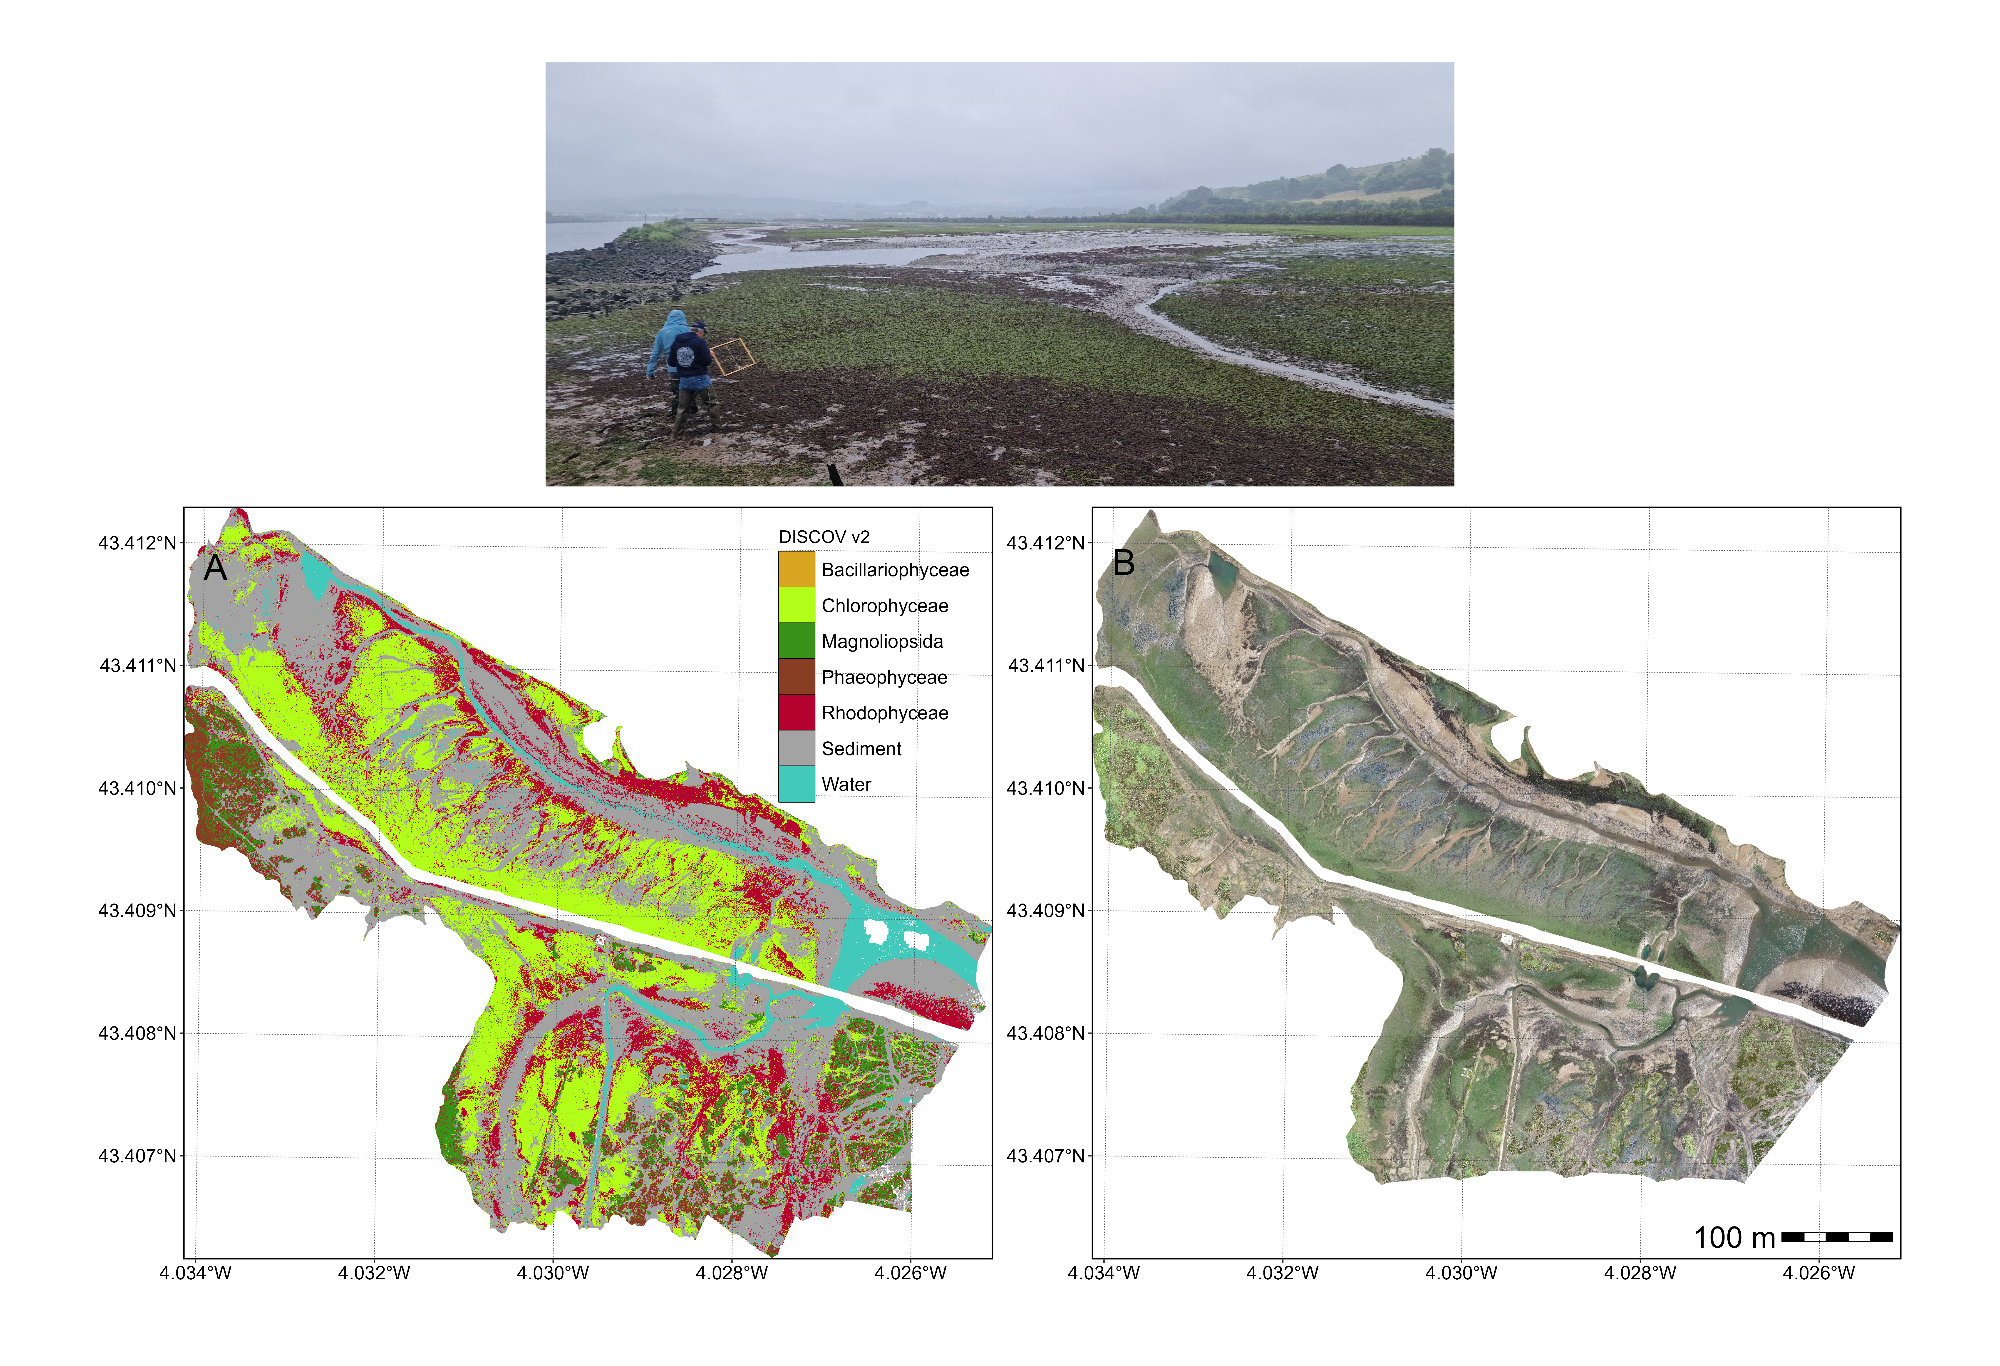
\includegraphics[width=0.95\linewidth,height=\textheight,keepaspectratio]{./Figures/Low_res/Saja_maps.png}

}

\caption{\label{fig-Saja}DISCOV Prediction (A), RGB composition (B) and
picture of the field campaign of the Saja esturay, Nothern Spain. The
total extent of this flight was 20.4 hectars with a resolution of 8 mm
per pixel.}

\end{figure}%

\newpage

\section*{References}\label{references}
\addcontentsline{toc}{section}{References}

\phantomsection\label{refs}
\begin{CSLReferences}{1}{0}
\bibitem[\citeproctext]{ref-abreu2011nitrogen}
Abreu, M.H., Pereira, R., Buschmann, A., Sousa-Pinto, I., Yarish, C.,
2011. Nitrogen uptake responses of gracilaria vermiculophylla (ohmi)
papenfuss under combined and single addition of nitrate and ammonium.
Journal of Experimental Marine Biology and Ecology 407, 190--199.

\bibitem[\citeproctext]{ref-agisoft}
Agisoft, 2019. \href{https://www.agisoft.com/}{Agisoft metashape}.

\bibitem[\citeproctext]{ref-arim2006spread}
Arim, M., Abades, S.R., Neill, P.E., Lima, M., Marquet, P.A., 2006.
Spread dynamics of invasive species. Proceedings of the National Academy
of Sciences 103, 374--378.

\bibitem[\citeproctext]{ref-bendor2006spatial}
BenDor, T.K., Metcalf, S.S., 2006. The spatial dynamics of invasive
species spread. System Dynamics Review: The Journal of the System
Dynamics Society 22, 27--50.

\bibitem[\citeproctext]{ref-besterman2021predicting}
Besterman, A.F., McGlathery, K.J., Reidenbach, M.A., Wiberg, P.L., Pace,
M.L., 2021. Predicting benthic macroalgal abundance in shallow coastal
lagoons from geomorphology and hydrologic flow patterns. Limnology and
Oceanography 66, 123--140.

\bibitem[\citeproctext]{ref-Blanchet2014}
Blanchet, H., Gouillieux, B., Alizier, S., others, 2014. Multiscale
patterns in the diversity and organization of benthic intertidal fauna
among french atlantic estuaries. Journal of Sea Research 90, 95--110.
\url{https://doi.org/10.1016/j.seares.2014.02.014}

\bibitem[\citeproctext]{ref-brunier2022evolution}
Brunier, G., Tamura, T., Anthony, E.J., Dussouillez, P., Gardel, A.,
2022. Evolution of the french guiana coast from late pleistocene to
holocene based on chenier and beach sand dating. Regional Environmental
Change 22, 122.

\bibitem[\citeproctext]{ref-brm3}
Bürkner, P.-C., 2021. Bayesian item response modeling in {R} with {brms}
and {Stan}. Journal of Statistical Software 100, 1--54.
\url{https://doi.org/10.18637/jss.v100.i05}

\bibitem[\citeproctext]{ref-brm2}
Bürkner, P.-C., 2018. Advanced {Bayesian} multilevel modeling with the
{R} package {brms}. The R Journal 10, 395--411.
\url{https://doi.org/10.32614/RJ-2018-017}

\bibitem[\citeproctext]{ref-brm1}
Bürkner, P.-C., 2017. {brms}: An {R} package for {Bayesian} multilevel
models using {Stan}. Journal of Statistical Software 80, 1--28.
\url{https://doi.org/10.18637/jss.v080.i01}

\bibitem[\citeproctext]{ref-calleja2017long}
Calleja, F., Galván, C., Silió-Calzada, A., Juanes, J.A., Ondiviela, B.,
2017. Long-term analysis of zostera noltei: A retrospective approach for
understanding seagrasses' dynamics. Marine environmental research 130,
93--105.

\bibitem[\citeproctext]{ref-Castaing1995}
Castaing, P., Guilcher, A., 1995. Morphosedimentary evolution of
ria-type estuaries. Earth Surface Processes and Landforms 20, 361--376.
\url{https://doi.org/10.1002/esp.3290200408}

\bibitem[\citeproctext]{ref-chadwick2020integrating}
Chadwick, K.D., Brodrick, P.G., Grant, K., Goulden, T., Henderson, A.,
Falco, N., Wainwright, H., Williams, K.H., Bill, M., Breckheimer, I.,
others, 2020. Integrating airborne remote sensing and field campaigns
for ecology and earth system science. Methods in Ecology and Evolution
11, 1492--1508.

\bibitem[\citeproctext]{ref-chand2021low}
Chand, S., Bollard, B., 2021. Low altitude spatial assessment and
monitoring of intertidal seagrass meadows beyond the visible spectrum
using a remotely piloted aircraft system. Estuarine, Coastal and Shelf
Science 255, 107299.

\bibitem[\citeproctext]{ref-shinypck}
Chang, W., Cheng, J., Allaire, J., Sievert, C., Schloerke, B., Xie, Y.,
Allen, J., McPherson, J., Dipert, A., Borges, B., 2024.
\href{https://CRAN.R-project.org/package=shiny}{Shiny: Web application
framework for r}.

\bibitem[\citeproctext]{ref-crowl2008spread}
Crowl, T.A., Crist, T.O., Parmenter, R.R., Belovsky, G., Lugo, A.E.,
2008. The spread of invasive species and infectious disease as drivers
of ecosystem change. Frontiers in Ecology and the Environment 6,
238--246.

\bibitem[\citeproctext]{ref-davies2023multi}
Davies, B.F.R., Gernez, P., Geraud, A., Oiry, S., Rosa, P., Zoffoli,
M.L., Barillé, L., 2023. Multi-and hyperspectral classification of
soft-bottom intertidal vegetation using a spectral library for coastal
biodiversity remote sensing. Remote Sensing of Environment 290, 113554.

\bibitem[\citeproctext]{ref-davies2024sentinel}
Davies, B.F.R., Oiry, S., Rosa, P., Zoffoli, M.L., Sousa, A.I., Thomas,
O.R., Smale, D.A., Austen, M.C., Biermann, L., Attrill, M.J., others,
2024b. A sentinel watching over inter-tidal seagrass phenology across
western europe and north africa. Communications Earth \& Environment 5,
382.

\bibitem[\citeproctext]{ref-davies2024intertidal}
Davies, B.F.R., Oiry, S., Rosa, P., Zoffoli, M.L., Sousa, A.I., Thomas,
O.R., Smale, D.A., Austen, M.C., Biermann, L., Attrill, M.J., others,
2024a. Intertidal seagrass extent from sentinel-2 time-series show
distinct trajectories in western europe. Remote Sensing of Environment
312, 114340.

\bibitem[\citeproctext]{ref-davoult2017multiple}
Davoult, D., Surget, G., Stiger-Pouvreau, V., Noisette, F., Riera, P.,
Stagnol, D., Androuin, T., Poupart, N., 2017. Multiple effects of a
gracilaria vermiculophylla invasion on estuarine mudflat functioning and
diversity. Marine Environmental Research 131, 227--235.

\bibitem[\citeproctext]{ref-rs14133124}
Diruit, W., Le Bris, A., Bajjouk, T., Richier, S., Helias, M., Burel,
T., Lennon, M., Guyot, A., Ar Gall, E., 2022. Seaweed habitats on the
shore: Characterization through hyperspectral UAV imagery and field
sampling. Remote Sensing 14. \url{https://doi.org/10.3390/rs14133124}

\bibitem[\citeproctext]{ref-rs14020346}
Douay, F., Verpoorter, C., Duong, G., Spilmont, N., Gevaert, F., 2022.
New hyperspectral procedure to discriminate intertidal macroalgae.
Remote Sensing 14. \url{https://doi.org/10.3390/rs14020346}

\bibitem[\citeproctext]{ref-douglas2024linking}
Douglas, T.J., Coops, N.C., Drever, M.C., Hunt, B.P., Martin, T.G.,
2024. Linking microphytobenthos distribution and mudflat geomorphology
under varying sedimentary regimes using unoccupied aerial vehicle
(UAV)-acquired multispectral reflectance and photogrammetry. Science of
The Total Environment 173675.

\bibitem[\citeproctext]{ref-duffy2018spatial}
Duffy, J.P., Pratt, L., Anderson, K., Land, P.E., Shutler, J.D., 2018.
Spatial assessment of intertidal seagrass meadows using optical imaging
systems and a lightweight drone. Estuarine, Coastal and Shelf Science
200, 169--180.

\bibitem[\citeproctext]{ref-elton2020ecology}
Elton, C.S., 2020. The ecology of invasions by animals and plants.
Springer Nature.

\bibitem[\citeproctext]{ref-firth2024invasive}
Firth, L.B., Foggo, A., Watts, T., Knights, A.M., DeAmicis, S., 2024.
Invasive macroalgae in native seagrass beds: Vectors of spread and
impacts. Annals of Botany 133, 41--50.

\bibitem[\citeproctext]{ref-gallardo2016global}
Gallardo, B., Clavero, M., Sánchez, M.I., Vilà, M., 2016. Global
ecological impacts of invasive species in aquatic ecosystems. Global
change biology 22, 151--163.

\bibitem[\citeproctext]{ref-van2018global}
Ginneken, V. van, Vries, E. de, others, 2018. The global dispersal of
the non-endemic invasive red alga gracilaria vermiculophylla in the
ecosystems of the euro-asia coastal waters including the wadden sea
unesco world heritage coastal area: Awful or awesome? Oceanography \&
Fisheries Open Access Journal 8, 4--26.

\bibitem[\citeproctext]{ref-green2021functional}
Green, S.J., Grosholz, E.D., 2021. Functional eradication as a framework
for invasive species control. Frontiers in Ecology and the Environment
19, 98--107.

\bibitem[\citeproctext]{ref-grizel1991introduction}
Grizel, H., Heral, M., 1991. Introduction into france of the japanese
oyster (crassostrea gigas). ICES Journal of Marine Science 47, 399--403.

\bibitem[\citeproctext]{ref-gurgel2018systematics}
Gurgel, C.F.D., Norris, J.N., Schmidt, W.E., Le, H.N., Fredericq, S.,
2018. Systematics of the gracilariales (rhodophyta) including new
subfamilies, tribes, subgenera, and two new genera, agarophyton gen.
Nov. And crassa gen. nov. Phytotaxa 374, 1--23.

\bibitem[\citeproctext]{ref-terrapck}
Hijmans, R.J., 2024.
\href{https://CRAN.R-project.org/package=terra}{Terra: Spatial data
analysis}.

\bibitem[\citeproctext]{ref-RemonterLeTempsIGN}
IGN, 2024. Remonter le temps.

\bibitem[\citeproctext]{ref-jones2021use}
Jones, P.E., Tummers, J.S., Galib, S.M., Woodford, D.J., Hume, J.B.,
Silva, L.G., Braga, R.R., Garcia de Leaniz, C., Vitule, J.R., Herder,
J.E., others, 2021. The use of barriers to limit the spread of aquatic
invasive animal species: A global review. Frontiers in Ecology and
Evolution 9, 611631.

\bibitem[\citeproctext]{ref-krueger2017genetic}
Krueger-Hadfield, S.A., Kollars, N.M., Strand, A.E., Byers, J.E.,
Shainker, S.J., Terada, R., Greig, T.W., Hammann, M., Murray, D.C.,
Weinberger, F., others, 2017. Genetic identification of source and
likely vector of a widespread marine invader. Ecology and evolution 7,
4432--4447.

\bibitem[\citeproctext]{ref-d15020161}
Massé, C., Viard, F., Humbert, S., Antajan, E., Auby, I., Bachelet, G.,
Bernard, G., Bouchet, V.M.P., Burel, T., Dauvin, J.-C., Delegrange, A.,
Derrien-Courtel, S., Droual, G., Gouillieux, B., Goulletquer, P.,
Guérin, L., Janson, A.-L., Jourde, J., Labrune, C., Lavesque, N.,
Leclerc, J.-C., Le Duff, M., Le Garrec, V., Noël, P., Nowaczyk, A.,
Pergent-Martini, C., Pezy, J.-P., Raoux, A., Raybaud, V., Ruitton, S.,
Sauriau, P.-G., Spilmont, N., Thibault, D., Vincent, D., Curd, A., 2023.
An overview of marine non-indigenous species found in three contrasting
biogeographic metropolitan french regions: Insights on distribution,
origins and pathways of introduction. Diversity 15.
\url{https://doi.org/10.3390/d15020161}

\bibitem[\citeproctext]{ref-rs11060704}
Mcilwaine, B., Casado, M.R., Leinster, P., 2019. Using 1st derivative
reflectance signatures within a remote sensing framework to identify
macroalgae in marine environments. Remote Sensing 11.
\url{https://doi.org/10.3390/rs11060704}

\bibitem[\citeproctext]{ref-jmse11020367}
Mendoza-Segura, C., Fernández, E., Beca-Carretero, P., 2023. Predicted
changes in the biogeographical range of gracilaria vermiculophylla under
present and future climate scenarios. Journal of Marine Science and
Engineering 11. \url{https://doi.org/10.3390/jmse11020367}

\bibitem[\citeproctext]{ref-Michel2021}
Michel, G., Le Bot, S., Lesourd, S., Lafite, R., 2021.
Morpho-sedimentological and dynamic patterns in a ria type estuary: The
belon estuary (south brittany, france). Journal of Maps 17, 389--400.
\url{https://doi.org/10.1080/17445647.2021.1925170}

\bibitem[\citeproctext]{ref-mudd2010does}
Mudd, S.M., D'Alpaos, A., Morris, J.T., 2010. How does vegetation affect
sedimentation on tidal marshes? Investigating particle capture and
hydrodynamic controls on biologically mediated sedimentation. Journal of
Geophysical Research: Earth Surface 115.

\bibitem[\citeproctext]{ref-nebel2020review}
Nebel, S., Beege, M., Schneider, S., Rey, G.D., 2020. A review of
photogrammetry and photorealistic 3D models in education from a
psychological perspective, in: Frontiers in Education. Frontiers Media
SA, p. 144.

\bibitem[\citeproctext]{ref-nyberg2007introduced}
Nyberg, C.D., 2007. Introduced marine macroalgae and habitat modifiers:
Their ecological role and significant attributes. Department of Marine
Ecology.

\bibitem[\citeproctext]{ref-nyberg2009flora}
Nyberg, C.D., Thomsen, M.S., Wallentinus, I., 2009. Flora and fauna
associated with the introduced red alga gracilaria vermiculophylla.
European Journal of Phycology 44, 395--403.

\bibitem[\citeproctext]{ref-ohmi1956contributions}
OHMI, H., 1956. CONTRIBUTIONS TO THE KNOWLEDGE OF GRACILARIACEAE FROM
JAPAN: Ⅱ. On a new species of the genus gracilariopsis, with some
considerations on its ecology. 北海道大學水産學部研究彙報 6, 271--279.

\bibitem[\citeproctext]{ref-rs16234383}
Oiry, S., Davies, B.F.R., Sousa, A.I., Rosa, P., Zoffoli, M.L., Brunier,
G., Gernez, P., Barillé, L., 2024. Discriminating seagrasses from green
macroalgae in european intertidal areas using high-resolution
multispectral drone imagery. Remote Sensing 16.
\url{https://doi.org/10.3390/rs16234383}

\bibitem[\citeproctext]{ref-olmedo2020far}
Olmedo-Masat, O.M., Raffo, M.P., Rodrı́guez-Pérez, D., Arijón, M.,
Sánchez-Carnero, N., 2020. How far can we classify macroalgae remotely?
An example using a new spectral library of species from the south west
atlantic (argentine patagonia). Remote Sensing 12, 3870.

\bibitem[\citeproctext]{ref-ortega2005fluxes}
Ortega, T., Ponce, R., Forja, J., Gómez-Parra, A., 2005. Fluxes of
dissolved inorganic carbon in three estuarine systems of the cantabrian
sea (north of spain). Journal of Marine Systems 53, 125--142.

\bibitem[\citeproctext]{ref-WoRMS303450}
Papenfuss, G.F., 1967.
\href{https://marinespecies.org/aphia.php?p=sourcedetails&id=303450}{Notes
on algal nomenclature - v. Various chlorophyceae and rhodophyceae}.
Phykos 5, 95--105.

\bibitem[\citeproctext]{ref-peidro2024quantifying}
Peidro-Devesa, M.J., Martı́nez-Movilla, A., Rodrı́guez-Somoza, J.L.,
Sánchez, J.M., Román, M., 2024. Quantifying intertidal macroalgae stocks
in the NW iberian peninsula using unmanned aerial vehicle (UAV)
multispectral imagery. Regional Studies in Marine Science 103621.

\bibitem[\citeproctext]{ref-ramus2017invasive}
Ramus, A.P., Silliman, B.R., Thomsen, M.S., Long, Z.T., 2017. An
invasive foundation species enhances multifunctionality in a coastal
ecosystem. Proceedings of the national academy of sciences 114,
8580--8585.

\bibitem[\citeproctext]{ref-roca2022monitoring}
Roca, M., Dunbar, M.B., Román, A., Caballero, I., Zoffoli, M.L., Gernez,
P., Navarro, G., 2022. Monitoring the marine invasive alien species
rugulopteryx okamurae using unmanned aerial vehicles and satellites.
Frontiers in Marine Science 9, 1004012.

\bibitem[\citeproctext]{ref-roman2024mapping}
Román, A., Oiry, S., Davies, B.F., Rosa, P., Gernez, P., Tovar-Sánchez,
A., Navarro, G., Méléder, V., Barillé, L., 2024. Mapping intertidal
microphytobenthic biomass with very high-resolution remote sensing
imagery in an estuarine system. Science of The Total Environment 177025.

\bibitem[\citeproctext]{ref-roman2021using}
Román, A., Tovar-Sánchez, A., Olivé, I., Navarro, G., 2021. Using a
UAV-mounted multispectral camera for the monitoring of marine
macrophytes. Frontiers in Marine Science 8, 722698.

\bibitem[\citeproctext]{ref-romero2008sintering}
Romero, M., Andrés, A., Alonso, R., Viguri, J., Rincón, J.M., 2008.
Sintering behaviour of ceramic bodies from contaminated marine
sediments. Ceramics International 34, 1917--1924.

\bibitem[\citeproctext]{ref-rueness2005life}
Rueness, J., 2005. Life history and molecular sequences of gracilaria
vermiculophylla (gracilariales, rhodophyta), a new introduction to
european waters. Phycologia 44, 120--128.

\bibitem[\citeproctext]{ref-savitzky1964smoothing}
Savitzky, A., Golay, M.J., 1964. Smoothing and differentiation of data
by simplified least squares procedures. Analytical chemistry 36,
1627--1639.

\bibitem[\citeproctext]{ref-sfriso2012spreading}
Sfriso, A., Wolf, M.A., Maistro, S., Sciuto, K., Moro, I., 2012.
Spreading and autoecology of the invasive species gracilaria
vermiculophylla (gracilariales, rhodophyta) in the lagoons of the
north-western adriatic sea (mediterranean sea, italy). Estuarine,
Coastal and Shelf Science 114, 192--198.

\bibitem[\citeproctext]{ref-simberloff2021maintenance}
Simberloff, D., 2021. Maintenance management and eradication of
established aquatic invaders. Hydrobiologia 848, 2399--2420.

\bibitem[\citeproctext]{ref-Simon2024ShinyApp}
Simon, O., 2024.
\href{https://oirysimon.shinyapps.io/shiny_validate/}{Shiny app for
validation dataset building}.

\bibitem[\citeproctext]{ref-sotka2018combining}
Sotka, E.E., Baumgardner, A.W., Bippus, P.M., Destombe, C., Duermit,
E.A., Endo, H., Flanagan, B.A., Kamiya, M., Lees, L.E., Murren, C.J.,
others, 2018. Combining niche shift and population genetic analyses
predicts rapid phenotypic evolution during invasion. Evolutionary
Applications 11, 781--793.

\bibitem[\citeproctext]{ref-surget2017processus}
Surget, G., 2017. Processus adaptatifs des v{é}g{é}taux marins face au
changement climatique {à} diff{é}rentes {é}chelles de temps et d'espace:
Dynamique de populations, m{é}tabolomique, {é}cophysiologie et
potentiels de valorisation (PhD thesis). Universit{é} de Bretagne
occidentale-Brest.

\bibitem[\citeproctext]{ref-Tankoua2011}
Tankoua, O.F., Buffet, P.-E., Amiard, J.-C., Amiard-Triquet, C.,
Mouneyrac, C., Berthet, B., 2011. Potential influence of confounding
factors (size, salinity) on biomarkers in the sentinel species
scrobicularia plana used in programmes monitoring estuarine quality.
Environmental Science and Pollution Research 18, 1253--1263.
\url{https://doi.org/10.1007/s11356-011-0479-3}

\bibitem[\citeproctext]{ref-terada2002review}
Terada, R., Yamamoto, H., 2002. Review of gracilaria vermiculophylla
(ohmi) papenfuss and other species in japan and asia. Taxonomy of
economic seaweeds, with special reference to Pacific species 8,
225--230.

\bibitem[\citeproctext]{ref-thomsen2009distribution}
Thomsen, M.S., McGlathery, K., Schwarzschild, A., Silliman, B., 2009.
Distribution and ecological role of the non-native macroalga gracilaria
vermiculophylla in virginia salt marshes. Biological Invasions 11,
2303--2316.

\bibitem[\citeproctext]{ref-thomsen2007gracilaria}
Thomsen, M.S., Staehr, P.A., Nyberg, C.D., Schwærter, S., Krause-Jensen,
D., Silliman, B.R., 2007. Gracilaria vermiculophylla (ohmi) papenfuss,
1967 (rhodophyta, gracilariaceae) in northern europe, with emphasis on
danish conditions, and what to expect in the future. Aquatic invasions
2, 83--94.

\bibitem[\citeproctext]{ref-thomsen2013effects}
Thomsen, M.S., Stæhr, P.A., Nejrup, L., Schiel, D.R., 2013. Effects of
the invasive macroalgae gracilaria vermiculophylla on two co-occurring
foundation species and associated invertebrates. Aquatic Invasions 8,
133--145.

\bibitem[\citeproctext]{ref-valle2015mapping}
Valle, M., Pala, V., Lafon, V., Dehouck, A., Garmendia, J.M., Borja, A.,
Chust, G., 2015. Mapping estuarine habitats using airborne hyperspectral
imagery, with special focus on seagrass meadows. Estuarine, Coastal and
Shelf Science 164, 433--442.

\bibitem[\citeproctext]{ref-van2003reintroduction}
Van Katwijk, M., 2003. Reintroduction of eelgrass (zostera marina l.) in
the dutch wadden sea: A research overview and management vision, in:
Challenges to the Wadden Sea Area. In: Proceedings of the 10th
International Scientific Wadden Sea Symposium, Groningen, the
Netherlands. pp. 173--195.

\bibitem[\citeproctext]{ref-weinberger2008invasive}
Weinberger, F., Buchholz, B., Karez, R., Wahl, M., 2008. The invasive
red alga gracilaria vermiculophylla in the baltic sea: Adaptation to
brackish water may compensate for light limitation. Aquatic Biology 3,
251--264.

\bibitem[\citeproctext]{ref-williams2007global}
Williams, S.L., Smith, J.E., 2007. A global review of the distribution,
taxonomy, and impacts of introduced seaweeds. Annu. Rev. Ecol. Evol.
Syst. 38, 327--359.

\bibitem[\citeproctext]{ref-d14121077}
Zenetos, A., Tsiamis, K., Galanidi, M., Carvalho, N., Bartilotti, C.,
Canning-Clode, J., Castriota, L., Chainho, P., Comas-González, R.,
Costa, A.C., Dragičević, B., Dulčić, J., Faasse, M., Florin, A.-B.,
Gittenberger, A., Jakobsen, H., Jelmert, A., Kerckhof, F., Lehtiniemi,
M., Livi, S., Lundgreen, K., Macic, V., Massé, C., Mavrič, B., Naddafi,
R., Orlando-Bonaca, M., Petovic, S., Png-Gonzalez, L., Carbonell
Quetglas, A., Ribeiro, R.S., Cidade, T., Smolders, S., Stæhr, P.A.U.,
Viard, F., Outinen, O., 2022. Status and trends in the rate of
introduction of marine non-indigenous species in european seas.
Diversity 14. \url{https://doi.org/10.3390/d14121077}

\bibitem[\citeproctext]{ref-zoffoli2021decadal}
Zoffoli, M.L., Gernez, P., Godet, L., Peters, S., Oiry, S., Barillé, L.,
2021. Decadal increase in the ecological status of a north-atlantic
intertidal seagrass meadow observed with multi-mission satellite
time-series. Ecological Indicators 130, 108033.

\bibitem[\citeproctext]{ref-zoffoli2023remote}
Zoffoli, M.L., Gernez, P., Oiry, S., Godet, L., Dalloyau, S., Davies,
B.F.R., Barillé, L., 2023. Remote sensing in seagrass ecology: Coupled
dynamics between migratory herbivorous birds and intertidal meadows
observed by satellite during four decades. Remote Sensing in Ecology and
Conservation 9, 420--433.

\end{CSLReferences}




\end{document}
